\PassOptionsToPackage{unicode=true}{hyperref} % options for packages loaded elsewhere
\PassOptionsToPackage{hyphens}{url}
%
\documentclass[]{article}
\usepackage{lmodern}
\usepackage{amssymb,amsmath}
\usepackage{ifxetex,ifluatex}
\usepackage{fixltx2e} % provides \textsubscript
\ifnum 0\ifxetex 1\fi\ifluatex 1\fi=0 % if pdftex
  \usepackage[T1]{fontenc}
  \usepackage[utf8]{inputenc}
  \usepackage{textcomp} % provides euro and other symbols
\else % if luatex or xelatex
  \usepackage{unicode-math}
  \defaultfontfeatures{Ligatures=TeX,Scale=MatchLowercase}
\fi
% use upquote if available, for straight quotes in verbatim environments
\IfFileExists{upquote.sty}{\usepackage{upquote}}{}
% use microtype if available
\IfFileExists{microtype.sty}{%
\usepackage[]{microtype}
\UseMicrotypeSet[protrusion]{basicmath} % disable protrusion for tt fonts
}{}
\IfFileExists{parskip.sty}{%
\usepackage{parskip}
}{% else
\setlength{\parindent}{0pt}
\setlength{\parskip}{6pt plus 2pt minus 1pt}
}
\usepackage{hyperref}
\hypersetup{
            pdftitle={Proposta de Roteiro para Elaboração de Estudos de Impacto na Mobilidade (EIM)},
            pdfborder={0 0 0},
            breaklinks=true}
\urlstyle{same}  % don't use monospace font for urls
\usepackage[margin=1in]{geometry}
\usepackage{graphicx,grffile}
\makeatletter
\def\maxwidth{\ifdim\Gin@nat@width>\linewidth\linewidth\else\Gin@nat@width\fi}
\def\maxheight{\ifdim\Gin@nat@height>\textheight\textheight\else\Gin@nat@height\fi}
\makeatother
% Scale images if necessary, so that they will not overflow the page
% margins by default, and it is still possible to overwrite the defaults
% using explicit options in \includegraphics[width, height, ...]{}
\setkeys{Gin}{width=\maxwidth,height=\maxheight,keepaspectratio}
\setlength{\emergencystretch}{3em}  % prevent overfull lines
\providecommand{\tightlist}{%
  \setlength{\itemsep}{0pt}\setlength{\parskip}{0pt}}
\setcounter{secnumdepth}{0}
% Redefines (sub)paragraphs to behave more like sections
\ifx\paragraph\undefined\else
\let\oldparagraph\paragraph
\renewcommand{\paragraph}[1]{\oldparagraph{#1}\mbox{}}
\fi
\ifx\subparagraph\undefined\else
\let\oldsubparagraph\subparagraph
\renewcommand{\subparagraph}[1]{\oldsubparagraph{#1}\mbox{}}
\fi

% set default figure placement to htbp
\makeatletter
\def\fps@figure{htbp}
\makeatother

\usepackage{booktabs}
\usepackage{longtable}
\usepackage{array}
\usepackage{multirow}
\usepackage{wrapfig}
\usepackage{float}
\usepackage{colortbl}
\usepackage{pdflscape}
\usepackage{tabu}
\usepackage{threeparttable}
\usepackage{threeparttablex}
\usepackage[normalem]{ulem}
\usepackage{makecell}
\usepackage{xcolor}

\title{Proposta de Roteiro para Elaboração de Estudos de Impacto na Mobilidade
(EIM)}
\author{}
\date{\vspace{-2.5em}}

\begin{document}
\maketitle

{
\setcounter{tocdepth}{2}
\tableofcontents
}
Polos Geradores de Viagens (PGVs) são empreendimentos com capacidade de
geração de volumes expressivos de viagens para deslocamento de pessoas
ou cargas. De acordo com o Art. 93 do CTB, empreendimentos de grande
porte caracterizados como polos geradores de tráfego somente podem ser
aprovados após anuência do órgão ou entidade de trânsito com
circunscrição sobre a via (BRASIL, 1997). Durante as etapas de execução
e operação de grandes empreendimentos, os diferentes interessados
compartilham os mesmos objetivos em relação à segurança e eficiência dos
sistemas de transporte e mobilidade urbana, bem como a compatibilidade
com a política de desenvolvimento urbano. Nesse sentido, análises de
impacto de tráfego conduzidas de forma apropriada podem fornecer uma
base factual para suportar decisões acertadas em relação às janelas
temporais de mitigação de efeitos gerados por empreendimentos que
produzem e/ou atraem viagens e caracterizados como PGVs (DENATRAN,
2001), garantindo a qualidade e segurança dos deslocamentos e seu uso
sustentável (ONU, 2019, 2020) por meio de uma distribuição justa e
equitativa dos espaços de deslocamento (Licínio Portugal, 2012). Dessa
maneira, o município e responsáveis pelos PGVs devem promover
iniciativas alinhadas que garantam ao cidadão seu direito de ir e vir
através de deslocamentos seguros, e que promovam a qualidade de vida e
sustentabilidade (DENATRAN, 2001). Ainda que a municipalidade contribua
fornecendo diretrizes, informações e orientações necessárias para
elaboração de EIMs, é de responsabilidade do empreendedor a elaboração
do EIM e a coleta de dados necessária que caracterizem e descrevam a
influência de viagens geradas pelos PGVs no contexto total de viagens
nas áreas de influência (DENATRAN, 2001; Licínio Portugal, 2012). Desse
modo, os custos incorridos para elaboração do EIM e o ônus de medidas
resultantes dos impactos apontados pelo EIM são de responsabilidade do
empreendedor (\textbf{Plano Diretor}; Art. 56; Parágrafo Único, pag.
67)(DENATRAN, 2001). Este documento consolida as diretrizes gerais para
elaboração de EIMs de empreendimentos em \textbf{Nome do Município},
considerando as definições do Manual de Procedimentos para o Tratamento
de Polos Geradores de Tráfego (DENATRAN, 2001), e as diretrizes gerais
indicadas pelo município de \textbf{Nome do Município} em seu
\textbf{Plano Diretor}. Todo emprendimento que, de acordo com os
critérios estabelecidos pela \textbf{Secretaria de Mobilidade},
estiverem obrigados a elaborar seu EIM deverão considerar as definições
desse documento e solicitar ao órgão de trânsito competente as
diretrizes específicas ao emprendimento (caso existam) considerando as
peculiaridades do local e do empreendimento.\\
No município de \textbf{Nome do Município} os projetos objeto de EVU
(Estudo de Viabilidade Urbanística) são caracterizados como Projetos
Especiais de Impacto Urbano de 1º, 2º e 3º graus de acordo com os
artigos 55, 56, 59, 61 e 62 do \textbf{Plano Diretor}, sendo aqueles de
2º e 3º em sua maioria empreendimentos com características que requerem
a elaboração de EIM.Os EIMs são adotados em casos de implantação,
expansão ou mudança das finalidades de uso de PGVs etais estudos devem
considerar valores de referência mínimos de viagens geradas por hora
pico para que se defina o impacto dos mesmos. Dessa forma EIMs requerem
técnicas de previsão de demandas e análise de capacidade do sistema para
suportar tais condições. Por meio de tais analises e previsões os EIMs
devem avaliar a intensificação de congestionamentos (aumento dos tempos
de deslocamento), a deterioração das condições físicas da área de
influência (redução de conforto e segurança), os conflitos entre tráfego
de passagem e aquele associado ao empreendimento (dificuldade de acesso
a certas áreas), a demanda por áreas de estacionamento,
embarque/desembarque e carga/descarga (DENATRAN, 2001). Também devem ser
considerados os impactos sobre o transporte público (\textbf{Plano
Diretor}; Art. 56.; I, a e Art. 57; V, DENATRAN, 2001 4.2.3, pag.24) e
modais alternativos que promovam a sustentabilidade e a segurança dos
usuários da via (Licinio Portugal, 2012). Os EIMs, enquanto estudos
especializados, permitem determinar potenciais impactos gerados por PGV,
apontando benefícios gerados a serem maximizados e os impactos negativos
considerados como pontos críticos e as possíveis alternativas de
resolução dos mesmos (DENATRAN, 2001). Tais estudos respondem questões
relacionadas a impactos derivados da implantação de PGVs (Erika Cristine
Kneib, 2011), que consideram: • Condições atuais de tráfego •
Expectativa de condições futuras com e sem a existência do PGV • A
consideração de modais de maior produtividade social como modais ativos
e transporte público • Capacidade do modelo atual de mobilidade em
atender demandas futuras • Necessidades adicionais de
mobilidade/acessibilidade que garantam a manutenção do atual Nível de
Serviço (NS) para os diferentes modais • Recomendações de melhorias
viárias para acomodar demandas futuras de tráfego As respostas a essas
questões contribuem para que a administração pública possa avaliar a
conveniência dos PGTs e garantir que tais empreendimentos estejam
comprometidos com os interesses coletivos da região. Ao solicitar
diretrizes para o EIM a ser realizado o empreendedor já deve de antemão
fornecer documentos com o plano de edificação, destacando as finalidades
de uso, expectativa de geração de viagens e apontamento dos modelos e
fatores de cálculo para as estimativas de demanda -- valores esses que
poderão ser atualizados quando da elaboração do EIM. As melhorias a
serem executadas não necessariamente dependem apenas de resultados
apontados no EIM visando eliminar, mitigar ou compensar os efeitos
negativos identificados durante as fases de implantação/operação do
empreendimento, tais melhorias também podem ser solicitadas pelo órgão
gestor quando houver recomendações de melhorias necessárias à região
identificadas em documentos como plano diretor e afins (\textbf{Plano
Diretor}; Art. 55; § 1º, pag. 66), e ainda, quando houver evidentes
assimetrias no uso da estrutura viária no entorno do empreendimento
relacionadas à oferta e demanda de vagas de estacionamento, ou uso da
capacidade viária frente à demanda gerada pelo PGT conforme a (Tabela 1.
Regramento.) (DENATRAN, 2001). Dessa maneira, responsáveis por PGTs em
alinhamento com o órgão gestor de tráfego devem viabilizar os espaços
internos necessários para estacionamento, embarque/desembarque e carga e
descarga na área interna do empreendimento e garantir a melhor inserção
possível do empreendimento na malha viária do município, reduzindo a
perturbação no tráfego de passagem e o impacto na vizinhança ao garantir
que o empreendimento irá absorver internamente a demanda gerada e tratar
os conflitos externos gerados, bem como os problemas de acessibilidade
de veículos e pedestres, ao mesmo tempo que assegure operações de carga
e descarga em área específica do PGT. Os responsáveis pela elaboração de
EIMs deverão comprovar habilitação para realização de tais estudos.
Neste caso o técnico responsável deverá fornecer documento assinado
informando que se responsabiliza pela supervisão do estudo, atestando a
veracidade dos dados apresentados -- sob pena de responsabilização em
caso de má fé na apresentação de dados precários sem a devida menção de
qualquer limitação nas informações prestadas. Da mesma forma o órgão
competente se compromete em submeter os estudos encaminhados a um corpo
técnico habilitado e respaldado para análise de EIMs. Embora
responsáveis pela elaboração de EIMS e avaliadores de EIMS possuam
papeis e objetivos específicos, ambos devem se comprometer em seguir
critérios éticos e objetivos na condução de análises e revisões de EIMs
visando a obtenção de melhores soluções em segurança, mobilidade,
acessibilidade, conforto e preservação do ambiente circundante
(\textbf{Plano Diretor}; Art. 56; I, a). Os EIMs deverão obedecer às
normas ABNT de redação e demais exigências aplicadas pelo órgão
responsável. Ainda, todos os dados de estudos, modelagens, cálculos e
projetos deverão ser entregues de forma digital em documentos, mapas na
escala 1:1000, planilhas, e arquivos DWG e GIS. As medidas mitigadoras
previstas e entregues no Plano Funcional Viário deverão ser suficientes
para viabilizar o emprendimento quanto aos aspectos de mobilidade urbana
de acorco com o ICU 2003 no horizonte de projeto e 10 anos , de acordo
com os seguintes critérios. • Nos casos com nível de serviço atual de A
a C, todo impacto que apresente um quociente superior a 2 (dois) deverá
mitigar ou compensar tais efeitos e em casos em que o quociente for
superior a 4 (quatro), deverá obrigatoriamente mitigar os efeitos no
local em que foi identificada a variação do nível de serviço. • Nos
casos de ``A'' a ``D'' que ultrapassem o nível de serviço ``D'' com o
empreendimento, as medidas mitigadoras deverão garantir uma situação em
que o nível de serviço não ultrapasse ``D''. • Nos casos em que o nível
de serviço atual for ``D'', e com o empreendimento seja mantido o nível
``D'', mas com variação superior a 2 pontos percentuais, deverão ser
aplicadas mitigações. • Por fim, naqueles casos com nível de serviço
superior a ``D'' as medidas mitigadoras deverão assegurar no horizonte
futuro adotado um nível de serviço igual ao do cenário futuro sem o
empreendimento, desse modo variações superiores a 1 ponto percentual no
ICU deverão ser mitigadas Tabela 1.

Conforme o manual do DENATRAN, os impactos na circulação viária
resultantes da implantação de PGTs deverão ser analisados
sistematicamente e deverão apresentar tratamentos que considerem
simultaneamente os efeitos indesejáveis na segurança, mobilidade e
acessibilidade de pessoas e veículos. Tão somente após aprovados pelo
município os tratamentos mitigatórios e compensatórios adequados
relacionados às diretrizes gerais exigidas e aquelas condições
específicas relacionadas ao empreendimento em questão (dada por meio de
diretrizes específicas), o processo administrativo enquanto parecer
técnico de anuência para execução de obras, serviços e operação poderá
ser concluído (DENATRAN, 2001). Caso as condicionantes estabelecidas nas
diretrizes não sejam atendidas o EIM será devolvido ao responsável pelo
empreendimento para revisão, e tais atualizações se darão em iterações
com o órgão responsável pela avaliação de EIMs até que todas as
pendências sejam sanadas e o processo administrativo possa então ser
concluído. Cabe também ressaltar que o EIM constitui parcela das
obrigações do responsável pelo empreendimento, uma vez que o EIM é parte
do EVU e deverá estar de acordo com as propostas ambientais,
arquitetônicas, urbanísticas e viárias (DENATRAN, 2001), previstas no
EVU, de modo que toda alteração em qualquer das partes deverá ser
compatibilizada, a fim de fornecer um conjunto único.

~

{ Estrutura de EIMs}

~

\hypertarget{identificauxe7uxe3o-do-empreendimento-item-4.2.2-denatran-2001}{%
\section{-- Identificação do Empreendimento (Item 4.2.2 Denatran
2001)}\label{identificauxe7uxe3o-do-empreendimento-item-4.2.2-denatran-2001}}

\hypertarget{nome-do-empreendimento-razuxe3o-social-nome-fantasia}{%
\subsection{Nome do empreendimento / Razão Social / Nome
fantasia}\label{nome-do-empreendimento-razuxe3o-social-nome-fantasia}}

\hypertarget{identificauxe7uxe3onuxfameros-dos-processos-que-tramitam-na-pmpa---eu-expediente-uxfanico-e-sei-quando-houver}{%
\subsection{Identificação/Números dos processos que tramitam na PMPA -
EU (Expediente Único) e SEI (quando
houver)}\label{identificauxe7uxe3onuxfameros-dos-processos-que-tramitam-na-pmpa---eu-expediente-uxfanico-e-sei-quando-houver}}

\hypertarget{atividade-conforme-planodiretor}{%
\subsection{\texorpdfstring{Atividade (conforme
\textbf{PlanoDiretor})}{Atividade (conforme PlanoDiretor)}}\label{atividade-conforme-planodiretor}}

\hypertarget{objeto-da-proposta-construuxe7uxe3o-ampliauxe7uxe3o-modificauxe7uxe3o-de-uso-em-funcionamento}{%
\subsection{Objeto da proposta (construção, ampliação, modificação de
uso, em
funcionamento}\label{objeto-da-proposta-construuxe7uxe3o-ampliauxe7uxe3o-modificauxe7uxe3o-de-uso-em-funcionamento}}

\hypertarget{apresentar-todas-as-informauxe7uxf5es-contidas-na-planilha-de-controle-e-registro-de-acordo-com-o-evu-apresentado}{%
\subsection{Apresentar todas as informações contidas na Planilha de
Controle e Registro, de acordo com o EVU
apresentado}\label{apresentar-todas-as-informauxe7uxf5es-contidas-na-planilha-de-controle-e-registro-de-acordo-com-o-evu-apresentado}}

\hypertarget{fase-do-licenciamento}{%
\subsection{Fase do Licenciamento}\label{fase-do-licenciamento}}

\hypertarget{localizauxe7uxe3o}{%
\subsection{Localização}\label{localizauxe7uxe3o}}

\hypertarget{responsuxe1vel-legal-pelo-empreendimento}{%
\subsection{Responsável legal pelo
empreendimento}\label{responsuxe1vel-legal-pelo-empreendimento}}

\hypertarget{responsuxe1vel-tuxe9cnico-pelo-empreendimento}{%
\subsection{Responsável Técnico pelo
empreendimento}\label{responsuxe1vel-tuxe9cnico-pelo-empreendimento}}

\hypertarget{apresentauxe7uxe3o-de-responsuxe1vel-tuxe9cnico-pelo-eim-com-comprovauxe7uxe3o-de-habilitauxe7uxe3o}{%
\subsection{Apresentação de responsável técnico pelo EIM com comprovação
de
habilitação}\label{apresentauxe7uxe3o-de-responsuxe1vel-tuxe9cnico-pelo-eim-com-comprovauxe7uxe3o-de-habilitauxe7uxe3o}}

\hypertarget{cronograma-de-execuuxe7uxe3o-fases-de-desenvolvimento-quando-houver}{%
\subsection{Cronograma de execução (fases de desenvolvimento -- quando
houver)}\label{cronograma-de-execuuxe7uxe3o-fases-de-desenvolvimento-quando-houver}}

\hypertarget{restriuxe7uxf5es-de-circulauxe7uxe3o-geradas-durante-a-execuuxe7uxe3o-do-empreendimento}{%
\subsection{Restrições de circulação geradas durante a execução do
empreendimento}\label{restriuxe7uxf5es-de-circulauxe7uxe3o-geradas-durante-a-execuuxe7uxe3o-do-empreendimento}}

\hypertarget{entorno}{%
\subsection{Entorno}\label{entorno}}

\hypertarget{caracteruxedsticas-funcionais-geomuxe9tricas-e-fuxedsicas-das-vias-existentes-sentidos-de-circulauxe7uxe3o-movimentos-proibidos-numero-de-faixas-de-rolamento-regulamentauxe7uxe3o-de-estacionamentos-largura-de-vias-e-passeios-raios-de-curva-e-inclinauxe7uxe3o}{%
\subsubsection{Características funcionais, geométricas e físicas das
vias existentes (sentidos de circulação, movimentos proibidos, numero de
faixas de rolamento, regulamentação de estacionamentos, largura de vias
e passeios, raios de curva e
inclinação)}\label{caracteruxedsticas-funcionais-geomuxe9tricas-e-fuxedsicas-das-vias-existentes-sentidos-de-circulauxe7uxe3o-movimentos-proibidos-numero-de-faixas-de-rolamento-regulamentauxe7uxe3o-de-estacionamentos-largura-de-vias-e-passeios-raios-de-curva-e-inclinauxe7uxe3o}}

\hypertarget{localizauxe7ao-e-programauxe7uxe3o-de-semuxe1foros}{%
\subsubsection{Localizaçao e programação de
semáforos}\label{localizauxe7ao-e-programauxe7uxe3o-de-semuxe1foros}}

\hypertarget{pesquisa-sobre-projetos-de-modificauxe7uxe3o-do-sistema-viuxe1rio-de-outros-polos-geradores-pruxf3ximos}{%
\subsubsection{Pesquisa sobre projetos de modificação do sistema viário
de outros polos geradores
próximos}\label{pesquisa-sobre-projetos-de-modificauxe7uxe3o-do-sistema-viuxe1rio-de-outros-polos-geradores-pruxf3ximos}}

\hypertarget{descriuxe7uxe3o-das-atividades-desenvolvidas-ou-previstas-com-breve-histuxf3rico-para-empreendimentos-existentes-caracterizando-o-perfil-de-uso-do-solo-no-entorno-e-destacando-empreendimentos-que-possam-competir-por-viagens-geradas-para-a-regiuxe3o.}{%
\subsubsection{Descrição das atividades desenvolvidas ou previstas, /
com breve histórico para empreendimentos existentes, caracterizando o
perfil de uso do solo no entorno e destacando empreendimentos que possam
competir por viagens geradas para a
região.}\label{descriuxe7uxe3o-das-atividades-desenvolvidas-ou-previstas-com-breve-histuxf3rico-para-empreendimentos-existentes-caracterizando-o-perfil-de-uso-do-solo-no-entorno-e-destacando-empreendimentos-que-possam-competir-por-viagens-geradas-para-a-regiuxe3o.}}

\hypertarget{perfil-do-empreendimento}{%
\subsubsection{Perfil do
empreendimento}\label{perfil-do-empreendimento}}

\hypertarget{condiuxe7uxf5es-existentes-caracterizando-o-espauxe7o-atual}{%
\subsubsection{Condições existentes, caracterizando o espaço
atual}\label{condiuxe7uxf5es-existentes-caracterizando-o-espauxe7o-atual}}

\hypertarget{dimensuxf5es-uxe1rea-construuxedda-uxe1rea-computuxe1vel-vagas-de-estacionamento}{%
\subsubsection{Dimensões (área construída, área computável, vagas de
estacionamento)}\label{dimensuxf5es-uxe1rea-construuxedda-uxe1rea-computuxe1vel-vagas-de-estacionamento}}

\hypertarget{uxe1reas-e-dados-especuxedficos-que-fazem-referuxeancia-uxe0s-atividades-desenvolvidas-no-empreendimento-conforme-tipologia.}{%
\subsubsection{Áreas e dados específicos que fazem referência às
atividades desenvolvidas no empreendimento, conforme
tipologia.}\label{uxe1reas-e-dados-especuxedficos-que-fazem-referuxeancia-uxe0s-atividades-desenvolvidas-no-empreendimento-conforme-tipologia.}}

\hypertarget{visuxe3o-geral-do-projeto}{%
\subsubsection{Visão geral do projeto}\label{visuxe3o-geral-do-projeto}}

\hypertarget{projeto-do-empreendimento}{%
\subsubsection{Projeto do
Empreendimento}\label{projeto-do-empreendimento}}

\hypertarget{horuxe1rios-de-operauxe7uxe3o-e-picos-de-demanda}{%
\subsubsection{Horários de operação e picos de
demanda}\label{horuxe1rios-de-operauxe7uxe3o-e-picos-de-demanda}}

\hypertarget{uxe1rea-construuxedda-da-edificauxe7uxe3o}{%
\subsubsection{Área construída da
edificação}\label{uxe1rea-construuxedda-da-edificauxe7uxe3o}}

\hypertarget{uxe1rea-de-aproveitamento-uxe1rea-ocupada-do-terreno}{%
\subsubsection{Área de aproveitamento / Área ocupada do
terreno}\label{uxe1rea-de-aproveitamento-uxe1rea-ocupada-do-terreno}}

\hypertarget{caracteruxedsticas-socioeconuxf4micas-de-moradores-para-empreendimentos-residenciais}{%
\subsubsection{Características socioeconômicas de moradores (para
empreendimentos
residenciais)}\label{caracteruxedsticas-socioeconuxf4micas-de-moradores-para-empreendimentos-residenciais}}

~

\hypertarget{anuxe1lise-do-projeto-sob-a-uxf3tica-viuxe1ria-item-4.2.3-denatran-2001}{%
\section{-- Análise do projeto sob a ótica Viária (Item 4.2.3 Denatran
2001)}\label{anuxe1lise-do-projeto-sob-a-uxf3tica-viuxe1ria-item-4.2.3-denatran-2001}}

\hypertarget{croquis-de-interseuxe7uxf5es-significativas-na-uxe1rea-de-influuxeancia-direta}{%
\subsection{Croquis de interseções significativas na área de influência
direta}\label{croquis-de-interseuxe7uxf5es-significativas-na-uxe1rea-de-influuxeancia-direta}}

\hypertarget{oferta-dimensionamento-e-distribuiuxe7uxe3o-de-vagas-de-estacionamentos}{%
\subsection{Oferta, dimensionamento e distribuição de vagas de
estacionamentos}\label{oferta-dimensionamento-e-distribuiuxe7uxe3o-de-vagas-de-estacionamentos}}

\hypertarget{dimensionamento-e-distribuiuxe7uxe3o-de-uxe1reas-de-carga-e-descarga}{%
\subsection{Dimensionamento e distribuição de áreas de carga e
descarga}\label{dimensionamento-e-distribuiuxe7uxe3o-de-uxe1reas-de-carga-e-descarga}}

\hypertarget{adequauxe7uxe3o-de-acessos-especuxedficos-para-veuxedculos-de-emerguxeancia-aplicuxe1vel-a-empreendimentos-promotores-de-grandes-eventos-item-5.2.1-denatran-2001}{%
\subsection{Adequação de acessos específicos para veículos de emergência
(aplicável a empreendimentos promotores de grandes eventos) (Item 5.2.1
Denatran
2001)}\label{adequauxe7uxe3o-de-acessos-especuxedficos-para-veuxedculos-de-emerguxeancia-aplicuxe1vel-a-empreendimentos-promotores-de-grandes-eventos-item-5.2.1-denatran-2001}}

\hypertarget{localizauxe7uxe3o-dos-acessos}{%
\subsection{Localização dos
acessos}\label{localizauxe7uxe3o-dos-acessos}}

\hypertarget{explicauxe7uxe3o-geral-sobre-os-acessos}{%
\subsubsection{Explicação geral sobre os
acessos}\label{explicauxe7uxe3o-geral-sobre-os-acessos}}

\hypertarget{croquifigura-do-empreendimento-indicando-o-local-dos-acessos-de-pedestres-veuxedculos-leves-veuxedculos-de-carga-uxe1reas-de-embarque-e-desembarque-e-de-veuxedculos-de-emerguxeancia-de-serviuxe7o-etc}{%
\subsubsection{Croqui/Figura do empreendimento indicando o local dos
acessos de pedestres, veículos leves, veículos de carga, áreas de
embarque e desembarque e de veículos de emergência, de serviço,
etc}\label{croquifigura-do-empreendimento-indicando-o-local-dos-acessos-de-pedestres-veuxedculos-leves-veuxedculos-de-carga-uxe1reas-de-embarque-e-desembarque-e-de-veuxedculos-de-emerguxeancia-de-serviuxe7o-etc}}

\hypertarget{descriuxe7uxe3o-da-circulauxe7uxe3o-e-acessibilidade-de-pedestres-e-transporte-coletivo}{%
\subsection{Descrição da circulação e acessibilidade de Pedestres e
Transporte
Coletivo}\label{descriuxe7uxe3o-da-circulauxe7uxe3o-e-acessibilidade-de-pedestres-e-transporte-coletivo}}

\hypertarget{descriuxe7uxe3o-da-circulauxe7uxe3o-e-acessibilidade-de-bicicletas}{%
\subsection{Descrição da circulação e acessibilidade de
Bicicletas}\label{descriuxe7uxe3o-da-circulauxe7uxe3o-e-acessibilidade-de-bicicletas}}

\hypertarget{descriuxe7uxe3o-da-circulauxe7uxe3o-e-acessibilidade-de-veuxedculos-leves-e-motocicletas}{%
\subsection{Descrição da circulação e acessibilidade de Veículos Leves e
Motocicletas}\label{descriuxe7uxe3o-da-circulauxe7uxe3o-e-acessibilidade-de-veuxedculos-leves-e-motocicletas}}

\hypertarget{descriuxe7uxe3o-da-circulauxe7uxe3o-e-acessibilidade-de-veuxedculos-pesados}{%
\subsection{Descrição da circulação e acessibilidade de Veículos
Pesados}\label{descriuxe7uxe3o-da-circulauxe7uxe3o-e-acessibilidade-de-veuxedculos-pesados}}

\hypertarget{descriuxe7uxe3o-da-circulauxe7uxe3o-e-acessibilidade-de-tuxe1xi-veuxedculos-fretados-veuxedculos-especiais-e-uxe1rea-de-embarque-e-desembarque}{%
\subsubsection{Descrição da circulação e acessibilidade de Táxi,
Veículos Fretados, Veículos Especiais e Área de Embarque e
Desembarque}\label{descriuxe7uxe3o-da-circulauxe7uxe3o-e-acessibilidade-de-tuxe1xi-veuxedculos-fretados-veuxedculos-especiais-e-uxe1rea-de-embarque-e-desembarque}}

\hypertarget{recuos-viuxe1rios}{%
\subsubsection{Recuos viários}\label{recuos-viuxe1rios}}

\hypertarget{declividade-de-rampas}{%
\subsubsection{Declividade de rampas}\label{declividade-de-rampas}}

\hypertarget{raios-de-giro-nos-acessos-e-vias-de-circulauxe7uxe3o-internas}{%
\subsubsection{Raios de giro nos acessos e vias de circulação
internas}\label{raios-de-giro-nos-acessos-e-vias-de-circulauxe7uxe3o-internas}}

\hypertarget{vias-internas-de-circulauxe7uxe3o}{%
\subsubsection{Vias internas de
circulação}\label{vias-internas-de-circulauxe7uxe3o}}

\hypertarget{cancelas-de-controle-de-acesso-caracterizando-demanda-tempo-de-atendimento-e-uxe1rea-de-acumulauxe7uxe3o-item-5.2.1-denatran-2001}{%
\subsubsection{Cancelas de controle de acesso, caracterizando demanda,
tempo de atendimento e área de acumulação (Item 5.2.1 Denatran
2001)}\label{cancelas-de-controle-de-acesso-caracterizando-demanda-tempo-de-atendimento-e-uxe1rea-de-acumulauxe7uxe3o-item-5.2.1-denatran-2001}}

\hypertarget{descriuxe7uxe3o-da-sinalizauxe7uxe3o-das-vias-de-acesso}{%
\subsubsection{Descrição da sinalização das vias de
acesso}\label{descriuxe7uxe3o-da-sinalizauxe7uxe3o-das-vias-de-acesso}}

~

\hypertarget{anuxe1lise-do-espauxe7o-viuxe1rio-item-4.2.3-denatran-2001}{%
\section{-- Análise do Espaço Viário (Item 4.2.3 Denatran
2001)}\label{anuxe1lise-do-espauxe7o-viuxe1rio-item-4.2.3-denatran-2001}}

\hypertarget{delimitauxe7uxe3o-da-uxe1rea-de-influuxeancia-direta-caracterizado-pelas-vias-de-acesso-e-adjacentes}{%
\subsection{Delimitação da Área de Influência Direta (caracterizado
pelas vias de acesso e
adjacentes)}\label{delimitauxe7uxe3o-da-uxe1rea-de-influuxeancia-direta-caracterizado-pelas-vias-de-acesso-e-adjacentes}}

\hypertarget{caracterizauxe7uxe3o-do-plano-diretor-para-o-local-quando-houver}{%
\subsection{Caracterização do plano diretor para o local -- quando
houver}\label{caracterizauxe7uxe3o-do-plano-diretor-para-o-local-quando-houver}}

\hypertarget{principais-eixos-de-ligauxe7uxe3o-uxe0-uxe1rea-de-influuxeancia-direta}{%
\subsection{Principais eixos de ligação à área de influência
direta}\label{principais-eixos-de-ligauxe7uxe3o-uxe0-uxe1rea-de-influuxeancia-direta}}

\hypertarget{caracteruxedsticas-fuxedsicas-da-uxe1rea-de-influuxeancia-direta}{%
\subsection{Características físicas da área de influência
direta}\label{caracteruxedsticas-fuxedsicas-da-uxe1rea-de-influuxeancia-direta}}

\hypertarget{anuxe1lise-da-circulauxe7uxe3o-na-uxe1rea-de-influuxeancia-na-situauxe7uxe3o-sem-o-empreendimento}{%
\subsection{Análise da circulação na área de influência na situação sem
o
empreendimento}\label{anuxe1lise-da-circulauxe7uxe3o-na-uxe1rea-de-influuxeancia-na-situauxe7uxe3o-sem-o-empreendimento}}

\hypertarget{pesquisa-de-contagem-volumuxe9trica-de-veuxedculos-volumes-classificados}{%
\subsubsection{Pesquisa de contagem volumétrica de veículos (volumes
classificados)}\label{pesquisa-de-contagem-volumuxe9trica-de-veuxedculos-volumes-classificados}}

\hypertarget{informauxe7uxf5es-sobre-a-pesquisa-realizada-e-descriuxe7uxe3o-metodoluxf3gica}{%
\paragraph{Informações sobre a pesquisa realizada e descrição
metodológica}\label{informauxe7uxf5es-sobre-a-pesquisa-realizada-e-descriuxe7uxe3o-metodoluxf3gica}}

\hypertarget{identificauxe7uxe3o-da-fonte-de-dados-e-apresentauxe7uxe3o-de-planilhas}{%
\paragraph{Identificação da fonte de dados e apresentação de
planilhas}\label{identificauxe7uxe3o-da-fonte-de-dados-e-apresentauxe7uxe3o-de-planilhas}}

\hypertarget{croqui-apresentando-os-movimentos-encontrados-nos-picos}{%
\paragraph{Croqui apresentando os movimentos encontrados nos
picos}\label{croqui-apresentando-os-movimentos-encontrados-nos-picos}}

\hypertarget{identificauxe7uxe3o-dos-peruxedodos-de-pico-de-truxe1fego-no-entorno}{%
\paragraph{Identificação dos períodos de pico de tráfego no
entorno}\label{identificauxe7uxe3o-dos-peruxedodos-de-pico-de-truxe1fego-no-entorno}}

\hypertarget{identificauxe7uxe3o-das-uxe1reas-de-impacto-direto-no-truxe1fego-local-e-de-passagem}{%
\paragraph{Identificação das áreas de impacto direto no tráfego local e
de
passagem}\label{identificauxe7uxe3o-das-uxe1reas-de-impacto-direto-no-truxe1fego-local-e-de-passagem}}

\hypertarget{cuxe1lculo-de-capacidadenuxedvel-de-serviuxe7o-da-situauxe7uxe3o-atual-sem-o-empreendimento-e-futura-com-e-sem-o-empreendimento-com-uxeanfase-nas-vias-de-acesso-e-adjacentes}{%
\subsubsection{Cálculo de Capacidade/nível de serviço da situação atual
sem o empreendimento e futura com e sem o empreendimento, com ênfase nas
vias de acesso e
adjacentes}\label{cuxe1lculo-de-capacidadenuxedvel-de-serviuxe7o-da-situauxe7uxe3o-atual-sem-o-empreendimento-e-futura-com-e-sem-o-empreendimento-com-uxeanfase-nas-vias-de-acesso-e-adjacentes}}

\hypertarget{utilizar-metodologia-icu-e-hcm}{%
\paragraph{Utilizar metodologia ICU e
HCM}\label{utilizar-metodologia-icu-e-hcm}}

\hypertarget{anuxe1lise-da-circulauxe7uxe3o-na-uxe1rea-de-influuxeancia-na-situauxe7uxe3o-atual-com-o-empreendimento-e-horizonte-de-10-anos-considerar-expansuxe3o-demogruxe1fica-e-de-novos-empreendimentos-se-for-o-caso}{%
\subsection{Análise da circulação na área de influência na situação
atual com o empreendimento (e horizonte de 10 anos -- considerar
expansão demográfica e de novos empreendimentos se for o
caso)}\label{anuxe1lise-da-circulauxe7uxe3o-na-uxe1rea-de-influuxeancia-na-situauxe7uxe3o-atual-com-o-empreendimento-e-horizonte-de-10-anos-considerar-expansuxe3o-demogruxe1fica-e-de-novos-empreendimentos-se-for-o-caso}}

\hypertarget{aplicauxe7uxe3o-do-modelo-4-etapas}{%
\subsubsection{Aplicação do Modelo 4
Etapas}\label{aplicauxe7uxe3o-do-modelo-4-etapas}}

\hypertarget{gerauxe7uxe3o-de-viagens}{%
\paragraph{Geração de Viagens}\label{gerauxe7uxe3o-de-viagens}}

\hypertarget{divisuxe3o-modal}{%
\paragraph{Divisão Modal}\label{divisuxe3o-modal}}

\hypertarget{distribuiuxe7uxe3o-das-viagens}{%
\paragraph{Distribuição das
Viagens}\label{distribuiuxe7uxe3o-das-viagens}}

\hypertarget{alocauxe7uxe3o-das-viagens}{%
\paragraph{Alocação das Viagens}\label{alocauxe7uxe3o-das-viagens}}

\hypertarget{apresentauxe7uxe3o-dos-fluxos-somados-da-contagem-de-truxe1fego-e-da-alocauxe7uxe3o-por-pico}{%
\subsubsection{Apresentação dos fluxos somados da contagem de tráfego e
da alocação por
pico}\label{apresentauxe7uxe3o-dos-fluxos-somados-da-contagem-de-truxe1fego-e-da-alocauxe7uxe3o-por-pico}}

\hypertarget{apresentauxe7uxe3o-do-modelo-de-expansuxe3o-de-matrizes}{%
\subsubsection{Apresentação do modelo de expansão de
matrizes}\label{apresentauxe7uxe3o-do-modelo-de-expansuxe3o-de-matrizes}}

\hypertarget{cuxe1lculo-do-nuxedvel-de-serviuxe7o-da-situauxe7uxe3o-atual-com-o-empreendimento}{%
\subsubsection{Cálculo do nível de serviço da situação atual com o
empreendimento}\label{cuxe1lculo-do-nuxedvel-de-serviuxe7o-da-situauxe7uxe3o-atual-com-o-empreendimento}}

\hypertarget{utilizar-metodologia-icu-e-hcm-1}{%
\paragraph{Utilizar metodologia ICU e
HCM}\label{utilizar-metodologia-icu-e-hcm-1}}

\hypertarget{cuxe1lculo-do-nuxedvel-de-serviuxe7o-da-situauxe7uxe3o-futura-horizonte-de-10-anos-com-o-empreendimento}{%
\subsubsection{Cálculo do nível de serviço da situação futura (horizonte
de 10 anos) com o
empreendimento}\label{cuxe1lculo-do-nuxedvel-de-serviuxe7o-da-situauxe7uxe3o-futura-horizonte-de-10-anos-com-o-empreendimento}}

\hypertarget{utilizar-metodologia-icu-e-hcm-2}{%
\paragraph{Utilizar metodologia ICU e
HCM}\label{utilizar-metodologia-icu-e-hcm-2}}

\hypertarget{apresentauxe7uxe3o-do-modelo-de-projeuxe7uxe3o-dos-dados}{%
\paragraph{Apresentação do modelo de projeção dos
dados}\label{apresentauxe7uxe3o-do-modelo-de-projeuxe7uxe3o-dos-dados}}

\hypertarget{anuxe1lise-comparada-nos-nuxedveis-de-serviuxe7o-e-capacidade-viuxe1ria-das-principais-interseuxe7uxf5es-e-acessos}{%
\subsubsection{Análise comparada nos Níveis de Serviço e Capacidade
Viária das principais interseções e
acessos}\label{anuxe1lise-comparada-nos-nuxedveis-de-serviuxe7o-e-capacidade-viuxe1ria-das-principais-interseuxe7uxf5es-e-acessos}}

\hypertarget{avaliauxe7uxe3o-do-carregamento-das-principais-interseuxe7uxf5es-e-acessos-na-hora-pico-nos-diferentes-cenuxe1rios-considerados}{%
\subsubsection{Avaliação do carregamento das principais interseções e
acessos na hora pico, nos diferentes cenários
considerados}\label{avaliauxe7uxe3o-do-carregamento-das-principais-interseuxe7uxf5es-e-acessos-na-hora-pico-nos-diferentes-cenuxe1rios-considerados}}

\hypertarget{anuxe1lise-das-condiuxe7uxf5es-de-oferta-de-transporte-puxfablico-e-privado-e-das-condiuxe7uxf5es-de-operauxe7uxe3o-considerando-a-situauxe7uxe3o-atual-e-futura}{%
\section{Análise das condições de oferta de transporte público e privado
e das condições de operação considerando a situação atual e
futura}\label{anuxe1lise-das-condiuxe7uxf5es-de-oferta-de-transporte-puxfablico-e-privado-e-das-condiuxe7uxf5es-de-operauxe7uxe3o-considerando-a-situauxe7uxe3o-atual-e-futura}}

\hypertarget{anuxe1lise-das-condiuxe7uxf5es-de-circulauxe7uxe3o-de-modais-alternativos-sobretudo-aqueles-relacionados-uxe0-mobilidade-ativa}{%
\subsubsection{Análise das condições de circulação de modais
alternativos, sobretudo aqueles relacionados à mobilidade
ativa}\label{anuxe1lise-das-condiuxe7uxf5es-de-circulauxe7uxe3o-de-modais-alternativos-sobretudo-aqueles-relacionados-uxe0-mobilidade-ativa}}

\hypertarget{avaliauxe7uxe3o-das-condiuxe7uxf5es-de-acesso-e-circulauxe7uxe3o-de-veuxedculos-e-pedestres-no-interior-do-empreendimento-bem-como-no-entorno-considerando-sobretudo-as-interferuxeancias-acarretadas-ao-fluxo-de-passagem-considerando-as-condiuxe7uxf5es-vigentes-de-fluidez-e-seguranuxe7a}{%
\subsubsection{Avaliação das condições de acesso e circulação de
veículos e pedestres no interior do empreendimento, bem como no entorno,
considerando sobretudo as interferências acarretadas ao fluxo de
passagem, considerando as condições vigentes de fluidez e
segurança}\label{avaliauxe7uxe3o-das-condiuxe7uxf5es-de-acesso-e-circulauxe7uxe3o-de-veuxedculos-e-pedestres-no-interior-do-empreendimento-bem-como-no-entorno-considerando-sobretudo-as-interferuxeancias-acarretadas-ao-fluxo-de-passagem-considerando-as-condiuxe7uxf5es-vigentes-de-fluidez-e-seguranuxe7a}}

\hypertarget{apresentauxe7uxe3o-da-matriz-de-anuxe1lise-de-impactos-considerando-a-fase-de-ocorruxeancia-do-impacto-efeito-sobre-o-meio-magnitude-dos-impactos-e-medidas-de-mitigauxe7uxe3o-ou-reversibilidade}{%
\subsubsection{Apresentação da matriz de análise de impactos
considerando a fase de ocorrência do impacto, efeito sobre o meio,
magnitude dos impactos e medidas de mitigação ou
reversibilidade}\label{apresentauxe7uxe3o-da-matriz-de-anuxe1lise-de-impactos-considerando-a-fase-de-ocorruxeancia-do-impacto-efeito-sobre-o-meio-magnitude-dos-impactos-e-medidas-de-mitigauxe7uxe3o-ou-reversibilidade}}

~

\hypertarget{proposiuxe7uxe3o-de-medidas-item-4.2.4-denatran-2001}{%
\section{Proposição de Medidas (Item 4.2.4 Denatran
2001)}\label{proposiuxe7uxe3o-de-medidas-item-4.2.4-denatran-2001}}

\hypertarget{identificauxe7uxe3o-de-problemas-circulauxe7uxe3o-acessibilidade-e-seguranuxe7a-no-projeto-e-proposiuxe7uxf5es-de-soluuxe7uxf5es-internas-e-externas-ao-empreendimento}{%
\subsection{Identificação de problemas (circulação, acessibilidade e
segurança) no Projeto e proposições de soluções internas e externas ao
empreendimento}\label{identificauxe7uxe3o-de-problemas-circulauxe7uxe3o-acessibilidade-e-seguranuxe7a-no-projeto-e-proposiuxe7uxf5es-de-soluuxe7uxf5es-internas-e-externas-ao-empreendimento}}

\hypertarget{apresentauxe7uxe3o-dos-impactos-de-transiuxe7uxe3o-modal-quando-o-empreendimento-acarretar-mudanuxe7a-do-perfil-de-uso-do-solo}{%
\subsection{Apresentação dos impactos de transição modal quando o
empreendimento acarretar mudança do perfil de uso do
solo}\label{apresentauxe7uxe3o-dos-impactos-de-transiuxe7uxe3o-modal-quando-o-empreendimento-acarretar-mudanuxe7a-do-perfil-de-uso-do-solo}}

\hypertarget{apresentar-projeto-de-sinalizauxe7uxe3o-se-houver-estacionamento}{%
\subsection{Apresentar Projeto de Sinalização, se houver
estacionamento}\label{apresentar-projeto-de-sinalizauxe7uxe3o-se-houver-estacionamento}}

\hypertarget{apresentauxe7uxe3o-de-medidas-no-espauxe7o-viuxe1rio-externo-ao-empreendimento}{%
\subsection{Apresentação de Medidas no espaço viário, externo ao
empreendimento}\label{apresentauxe7uxe3o-de-medidas-no-espauxe7o-viuxe1rio-externo-ao-empreendimento}}

\hypertarget{proposiuxe7uxe3o-de-medidas-operacionais-ou-de-gerenciamento-do-truxe1fego-quando-cabuxedvel-visando-contribuir-na-melhoria-das-condiuxe7uxf5es-operacionais-sobretudo-aqueles-pgvs-que-em-funuxe7uxe3o-da-natureza-da-atividade-realizam-eventos-de-grande-porte-que-possam-sobrecarregar-o-sistema-viuxe1rio-requerendo-intervenuxe7uxe3o-direta-sobre-a-operauxe7uxe3o-da-via-em-datas-especuxedficas.}{%
\subsubsection{Proposição de medidas operacionais ou de gerenciamento do
tráfego (quando cabível) visando contribuir na melhoria das condições
operacionais -- sobretudo aqueles PGVs que em função da natureza da
atividade realizam eventos de grande porte que possam sobrecarregar o
sistema viário, requerendo intervenção direta sobre a operação da via em
datas
específicas.}\label{proposiuxe7uxe3o-de-medidas-operacionais-ou-de-gerenciamento-do-truxe1fego-quando-cabuxedvel-visando-contribuir-na-melhoria-das-condiuxe7uxf5es-operacionais-sobretudo-aqueles-pgvs-que-em-funuxe7uxe3o-da-natureza-da-atividade-realizam-eventos-de-grande-porte-que-possam-sobrecarregar-o-sistema-viuxe1rio-requerendo-intervenuxe7uxe3o-direta-sobre-a-operauxe7uxe3o-da-via-em-datas-especuxedficas.}}

\hypertarget{medidas-a-serem-tomadas-pelo-empreendedor-para-minimizar-os-impactos-causados-na-malha-urbana-da-cidade-pelo-empreendimento-tais-como}{%
\subsubsection{Medidas a serem tomadas pelo empreendedor para minimizar
os impactos causados na malha urbana da cidade pelo empreendimento, tais
como:}\label{medidas-a-serem-tomadas-pelo-empreendedor-para-minimizar-os-impactos-causados-na-malha-urbana-da-cidade-pelo-empreendimento-tais-como}}

\hypertarget{mudanuxe7a-de-sentido-de-truxe1fego}{%
\paragraph{Mudança de sentido de
tráfego}\label{mudanuxe7a-de-sentido-de-truxe1fego}}

\hypertarget{implantauxe7uxe3o-e-alargamento-de-vias}{%
\paragraph{Implantação e alargamento de
vias}\label{implantauxe7uxe3o-e-alargamento-de-vias}}

\hypertarget{implantauxe7uxe3o-de-obras-de-arte}{%
\paragraph{Implantação de obras de
arte}\label{implantauxe7uxe3o-de-obras-de-arte}}

\hypertarget{implantauxe7uxe3o-de-alterauxe7uxf5es-geomuxe9tricas}{%
\paragraph{Implantação de alterações
geométricas}\label{implantauxe7uxe3o-de-alterauxe7uxf5es-geomuxe9tricas}}

\hypertarget{implantauxe7uxe3o-de-melhorias-de-pavimentauxe7uxe3o}{%
\paragraph{Implantação de melhorias de
pavimentação}\label{implantauxe7uxe3o-de-melhorias-de-pavimentauxe7uxe3o}}

\hypertarget{implantauxe7uxe3o-manutenuxe7uxe3o-de-sinalizauxe7uxe3o-horizontal-vertical-e-semafuxf3rica}{%
\paragraph{Implantação / manutenção de sinalização horizontal, vertical
e
semafórica}\label{implantauxe7uxe3o-manutenuxe7uxe3o-de-sinalizauxe7uxe3o-horizontal-vertical-e-semafuxf3rica}}

\hypertarget{ajustes-na-programauxe7uxe3o-semafuxf3rica}{%
\paragraph{Ajustes na programação
semafórica}\label{ajustes-na-programauxe7uxe3o-semafuxf3rica}}

\hypertarget{implantauxe7uxe3o-de-medidas-moderadoras-de-truxe1fego}{%
\paragraph{Implantação de medidas moderadoras de
tráfego}\label{implantauxe7uxe3o-de-medidas-moderadoras-de-truxe1fego}}

\hypertarget{tratamento-para-pedestres-ciclistas-e-pessoas-com-deficiuxeancia-ou-mobilidade-reduzida}{%
\paragraph{Tratamento para pedestres, ciclistas e pessoas com
deficiência ou mobilidade
reduzida}\label{tratamento-para-pedestres-ciclistas-e-pessoas-com-deficiuxeancia-ou-mobilidade-reduzida}}

\hypertarget{recomendauxe7uxe3o-de-implantauxe7uxe3o-de-linhas-de-transporte-coletivo-escolar-ou-uxe1reas-para-embarque-e-desembarque-ou-tuxe1xi}{%
\paragraph{Recomendação de implantação de linhas de transporte coletivo,
escolar ou áreas para embarque e desembarque ou
táxi}\label{recomendauxe7uxe3o-de-implantauxe7uxe3o-de-linhas-de-transporte-coletivo-escolar-ou-uxe1reas-para-embarque-e-desembarque-ou-tuxe1xi}}

\hypertarget{propostas-de-fomento-uxe0-transiuxe7uxe3o-modal-como-oferta-de-infraestrutura-diferenciada-para-mobilidade-sustentuxe1vel}{%
\paragraph{Propostas de fomento à transição modal, como oferta de
infraestrutura diferenciada para mobilidade
sustentável}\label{propostas-de-fomento-uxe0-transiuxe7uxe3o-modal-como-oferta-de-infraestrutura-diferenciada-para-mobilidade-sustentuxe1vel}}

\hypertarget{proposiuxe7uxe3o-de-medidas-mitigatuxf3rias-quando-da-impossibilidade-de-mitigauxe7uxe3o-completa-dos-impactos-negativos}{%
\paragraph{Proposição de medidas mitigatórias quando da impossibilidade
de mitigação completa dos impactos
negativos}\label{proposiuxe7uxe3o-de-medidas-mitigatuxf3rias-quando-da-impossibilidade-de-mitigauxe7uxe3o-completa-dos-impactos-negativos}}

\hypertarget{plano-funcional-viuxe1rio-como-produto-final-do-eim-apresentando-projeto-buxe1sico-de-todas-as-intervenuxe7uxf5es-viuxe1rias-apresentadas-para-mitigar-os-impactos-do-pgv}{%
\paragraph{Plano Funcional Viário como produto final do EIM apresentando
projeto básico de todas as intervenções viárias apresentadas para
mitigar os impactos do
PGV}\label{plano-funcional-viuxe1rio-como-produto-final-do-eim-apresentando-projeto-buxe1sico-de-todas-as-intervenuxe7uxf5es-viuxe1rias-apresentadas-para-mitigar-os-impactos-do-pgv}}

\hypertarget{outras-medidas-cabuxedveis}{%
\paragraph{Outras medidas cabíveis}\label{outras-medidas-cabuxedveis}}

~

\hypertarget{medidas-futuras-de-seguranuxe7a-viuxe1ria-item-5.1-denatran-2001}{%
\section{Medidas Futuras de Segurança Viária (Item 5.1 Denatran
2001)}\label{medidas-futuras-de-seguranuxe7a-viuxe1ria-item-5.1-denatran-2001}}

\hypertarget{compromisso-de-avaliauxe7uxe3o-dos-uxedndices-de-acidentalidade-no-horizonte-de-3-a-5-anos}{%
\subsection{Compromisso de avaliação dos índices de acidentalidade no
horizonte de 3 a 5
anos}\label{compromisso-de-avaliauxe7uxe3o-dos-uxedndices-de-acidentalidade-no-horizonte-de-3-a-5-anos}}

\hypertarget{compromisso-de-proposiuxe7uxe3o-de-medidas-de-seguranuxe7a-viuxe1ria-quando-identificado-incremento-nos-uxedndices-de-acidentalidade-absolutos-e-uvp-superiores-uxe0-taxa-esperada-para-a-regiuxe3o-denatran-2001-pag-32}{%
\subsection{Compromisso de proposição de medidas de segurança viária
quando identificado incremento nos índices de acidentalidade absolutos e
UVP superiores à taxa esperada para a região (DENATRAN, 2001, pag
32)}\label{compromisso-de-proposiuxe7uxe3o-de-medidas-de-seguranuxe7a-viuxe1ria-quando-identificado-incremento-nos-uxedndices-de-acidentalidade-absolutos-e-uvp-superiores-uxe0-taxa-esperada-para-a-regiuxe3o-denatran-2001-pag-32}}

~

{ Informações Adicionais }

Projeção do Tráfego de Passagem:\\
Para estimar o tráfego futuro sem o empreendimento urbanístico, são
utilizadas taxas de crescimento para o tráfego atual. Na falta de
informações específicas, adota-se a taxa de 1,5\% ao ano, que é um valor
recomendado e utilizado para estudos de tráfego na Região Metropolitana
de \textbf{NomeDoMunicípio} (RMXX).\\
A situação futura com projeto é constituída da situação sem projeto
acrescida da demanda na situação com projeto. Com os dois cenários de
análise (situação futura sem projeto e com projeto), é feita uma
comparação dos níveis de serviço do sistema viário e são estabelecidos
os impactos.\\
Quando houver dados atualizados, oriundos de fontes de dados oficiais, o
responsável pelo estudo poderá sugerir para avaliação um cálculo de
projeção que julgue adequado, apresentando os dados e o modelo
matemático adotado. Após análise, a \textbf{SecretariaMobilidadeXX}
indicará se a proposta é aceitável ou se a projeção de 1,5\% deve ser
mantida.

~

{ Medidas Compensátórias }

Atualmente a \textbf{SecretariaMobilidadeXX} considera no entorno
imediato todas as interseçõs como nível \textbf{D}. Nesse caso,
empreendimentos com interseções em níveis \textbf{A}, \textbf{B} ou
\textbf{C} podem acumular demanda utilizando a capacidade atual desde
que não extrapolem o nível \textbf{D}, ou seja, um intervalo
correspondente à 68\% da capacidade. Esse modelo é bastante permissivo
para empreendimentos instalados em regiões com boas condições de
fluidez, ao mesmo tempo que é restritivo para aqueles casos com níveis
de serviço acima de \textbf{D}, já que estes devem garantir a manutenção
no nível de serviço pré-existente.

{ Critérios}

Diante disso, a proposta é de adotar a avaliação dos níveis de serviço
de \textbf{A} a \textbf{C} a partir do quociente entre a variação do ICU
sem projeto e a variação do ICU com projeto, nos horizontes de
inauguração do empreendimento e futuro (10 anos) desde que tais níveis
não alcancem o nível \textbf{D}. Desse modo:

\begin{itemize}
\tightlist
\item
  Nos casos com nível de serviço atual de \textbf{A} a \textbf{C}em que
  o quociente for superior a 4 (quatro), deverá obrigatoriamente mitigar
  os efeitos no local em que foi identificada a variação do nível de
  serviço.\\
\item
  Nos casos de \textbf{A} a \textbf{D} que ultrapassem o nível de
  serviço \textbf{D} com o empreendimento, as medidas mitigadoras
  deverão garantir uma situação em que o nível de serviço não ultrapasse
  \textbf{D}.
\item
  Nos casos em que o nível de serviço atual for \textbf{D}, e com o
  empreendimento seja mantido o nível \textbf{D}, mas com variação
  superior a 2 pontos percentuais, deverão ser aplicadas mitigações.\\
\item
  Por fim, naqueles casos com nível de serviço superior a \textbf{D} as
  medidas mitigadoras deverão assegurar no horizonte futuro adotado um
  nível de serviço igual ao do cenário futuro sem o empreendimento,
  desse modo variações superiores a 1 ponto percentual no ICU deverão
  ser mitigadas Tabela 1. A Figura 1 ilustra uma situação em que para
  aqueles cenários com ICU entre \textbf{A} e \textbf{C}, a regra da
  variação possa ser adotada.
\end{itemize}

\begin{table}

\caption{\label{tab:unnamed-chunk-1}Tabela 1. Regramento para compensações/mitigações.}
\centering
\begin{tabular}[t]{l|l|l|l|l|l}
\hline
Nível de Serviço & Atual & Sem empreendimento & Com Empreendimento & Quociente & Regra\\
\hline
[A, C] & ICU= 33\% & ICU=34\%, variação = 3,03\% & ICU=38+, variação = 15,15\% & 5 & Se >4, Mitigar no local de avaliação do Nível de Serviço\\
\hline
[A, C] & ICU= 61\% & ICU=62\%, variação = 1,64\% & ICU=63+, variação = 3,28\% & 2 & Se >=2, Compensar/Mitigar\\
\hline
[A, D] & [A, D] & [A, D] & Superior a D & - & Mitigar e garintir nível menor ou igual a D\\
\hline
D & D & D & D, com variação > 2 pontos percentuais & - & Mitigar para manter o nível de serviço menor ou igual ao percentual de capacidae atual\\
\hline
[E, H] & [E, H] & [E, H] & [E,a H] com Variação > 1 ponto percentual & - & Mitigar para manter o mesmo nível de serviço\\
\hline
\end{tabular}
\end{table}

Os valores exibidos na Tabela 1 foram obtidos de um cenário real
demonstrado na Figura 1.

Figura 1. Cenários reais ICU.\\

\begin{figure}
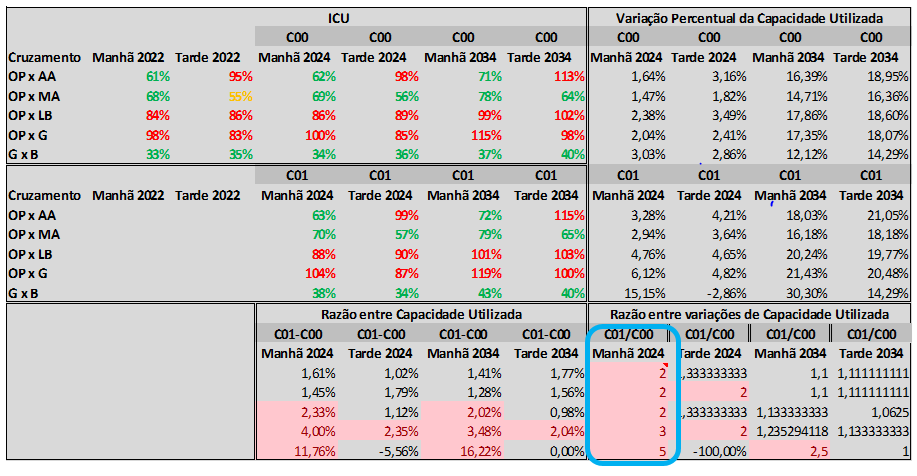
\includegraphics[width=1\linewidth]{CenarioICU} \end{figure}

 { Justificativa}

Justificativa: As vias são projetadas em um horizonte de projeto de 25 a
30 anos, assim, tais vias são projetadas para capacidades que consideram
o crescimento natural da demanda para o período que compõe o horizonte
de projeto. Dessa maneira, quando um empreendimento gera uma alavancagem
no crescimento que constitui o dobro do crescimento da demanda natural
(quociente 2), isso faz com que a vida útil da instalação seja
abreviada.\\
 Conforme ilustrado na Tabela 2, a coluna crescimento natural considera
um crescimento no volume de 1,5\% ao ano; já a coluna crescimento com
emprendimento apresenta a composição do crescimento natural da demanda
acrescida de um crescimento gerado pelo empreendimento totalizando um
crescimento da ordem de 2,65\% ao ano. No cenário que considera apenas o
crescimento natural a capacidade da instalação atenderia a demanda pelos
25 anos de projeto, sendo superada apenas no 26º ano; no cenário com
crescimento da demanda gerada com o empreendimento, a capacidade da
demanda de projeto seria atendida até o 14º ano apenas, abreviando a
vida útil de projeto em 11 anos.

\begin{table}

\caption{\label{tab:unnamed-chunk-3}Tabela 2. Evolução da Demamda até a capacidade de projeto de 1600 veiculos/hora.}
\centering
\begin{tabular}[t]{l|l|l}
\hline
Ano de Projeto & Crescimento Natural & Crescimento com Empreendimento\\
\hline
Ano 0 & \cellcolor[HTML]{4361ee}{\textcolor{white}{\textbf{1100}}} & \cellcolor[HTML]{4361ee}{\textcolor{white}{\textbf{1100}}}\\
\hline
Ano 1 & \cellcolor[HTML]{4361ee}{\textcolor{white}{\textbf{1116}}} & \cellcolor[HTML]{4361ee}{\textcolor{white}{\textbf{1129}}}\\
\hline
Ano 2 & \cellcolor[HTML]{4361ee}{\textcolor{white}{\textbf{1133}}} & \cellcolor[HTML]{4361ee}{\textcolor{white}{\textbf{1159}}}\\
\hline
Ano 3 & \cellcolor[HTML]{4361ee}{\textcolor{white}{\textbf{1150}}} & \cellcolor[HTML]{4361ee}{\textcolor{white}{\textbf{1189}}}\\
\hline
Ano 4 & \cellcolor[HTML]{4361ee}{\textcolor{white}{\textbf{1167}}} & \cellcolor[HTML]{4361ee}{\textcolor{white}{\textbf{1221}}}\\
\hline
Ano 5 & \cellcolor[HTML]{4361ee}{\textcolor{white}{\textbf{1185}}} & \cellcolor[HTML]{4361ee}{\textcolor{white}{\textbf{1253}}}\\
\hline
Ano 6 & \cellcolor[HTML]{4361ee}{\textcolor{white}{\textbf{1202}}} & \cellcolor[HTML]{4361ee}{\textcolor{white}{\textbf{1286}}}\\
\hline
Ano 7 & \cellcolor[HTML]{4361ee}{\textcolor{white}{\textbf{1220}}} & \cellcolor[HTML]{4361ee}{\textcolor{white}{\textbf{1321}}}\\
\hline
Ano 8 & \cellcolor[HTML]{4361ee}{\textcolor{white}{\textbf{1239}}} & \cellcolor[HTML]{4361ee}{\textcolor{white}{\textbf{1356}}}\\
\hline
Ano 9 & \cellcolor[HTML]{4361ee}{\textcolor{white}{\textbf{1257}}} & \cellcolor[HTML]{4361ee}{\textcolor{white}{\textbf{1391}}}\\
\hline
Ano 10 & \cellcolor[HTML]{4361ee}{\textcolor{white}{\textbf{1276}}} & \cellcolor[HTML]{4361ee}{\textcolor{white}{\textbf{1428}}}\\
\hline
Ano 11 & \cellcolor[HTML]{4361ee}{\textcolor{white}{\textbf{1295}}} & \cellcolor[HTML]{4361ee}{\textcolor{white}{\textbf{1466}}}\\
\hline
Ano 12 & \cellcolor[HTML]{4361ee}{\textcolor{white}{\textbf{1315}}} & \cellcolor[HTML]{4361ee}{\textcolor{white}{\textbf{1505}}}\\
\hline
Ano 13 & \cellcolor[HTML]{4361ee}{\textcolor{white}{\textbf{1334}}} & \cellcolor[HTML]{4361ee}{\textcolor{white}{\textbf{1545}}}\\
\hline
Ano 14 & \cellcolor[HTML]{4361ee}{\textcolor{white}{\textbf{1354}}} & \cellcolor[HTML]{4361ee}{\textcolor{white}{\textbf{1586}}}\\
\hline
Ano 15 & \cellcolor[HTML]{4361ee}{\textcolor{white}{\textbf{1375}}} & \cellcolor[HTML]{c1121f}{\textcolor{white}{\textbf{1628}}}\\
\hline
Ano 16 & \cellcolor[HTML]{4361ee}{\textcolor{white}{\textbf{1395}}} & \cellcolor[HTML]{c1121f}{\textcolor{white}{\textbf{1671}}}\\
\hline
Ano 17 & \cellcolor[HTML]{4361ee}{\textcolor{white}{\textbf{1416}}} & \cellcolor[HTML]{c1121f}{\textcolor{white}{\textbf{1715}}}\\
\hline
Ano 18 & \cellcolor[HTML]{4361ee}{\textcolor{white}{\textbf{1438}}} & \cellcolor[HTML]{c1121f}{\textcolor{white}{\textbf{1761}}}\\
\hline
Ano 19 & \cellcolor[HTML]{4361ee}{\textcolor{white}{\textbf{1459}}} & \cellcolor[HTML]{c1121f}{\textcolor{white}{\textbf{1808}}}\\
\hline
Ano 20 & \cellcolor[HTML]{4361ee}{\textcolor{white}{\textbf{1481}}} & \cellcolor[HTML]{c1121f}{\textcolor{white}{\textbf{1855}}}\\
\hline
Ano 21 & \cellcolor[HTML]{4361ee}{\textcolor{white}{\textbf{1503}}} & \cellcolor[HTML]{c1121f}{\textcolor{white}{\textbf{1905}}}\\
\hline
Ano 22 & \cellcolor[HTML]{4361ee}{\textcolor{white}{\textbf{1526}}} & \cellcolor[HTML]{c1121f}{\textcolor{white}{\textbf{1955}}}\\
\hline
Ano 23 & \cellcolor[HTML]{4361ee}{\textcolor{white}{\textbf{1549}}} & \cellcolor[HTML]{c1121f}{\textcolor{white}{\textbf{2007}}}\\
\hline
Ano 24 & \cellcolor[HTML]{4361ee}{\textcolor{white}{\textbf{1572}}} & \cellcolor[HTML]{c1121f}{\textcolor{white}{\textbf{2060}}}\\
\hline
Ano 25 & \cellcolor[HTML]{4361ee}{\textcolor{white}{\textbf{1596}}} & \cellcolor[HTML]{c1121f}{\textcolor{white}{\textbf{2115}}}\\
\hline
Ano 26 & \cellcolor[HTML]{c1121f}{\textcolor{white}{\textbf{1619}}} & \cellcolor[HTML]{c1121f}{\textcolor{white}{\textbf{2171}}}\\
\hline
\end{tabular}
\end{table}

{ Área de Influência }

\begin{table}

\caption{\label{tab:unnamed-chunk-4}Tabela 3. Áreas de Influencia Direta e Indireta em 118 cidades}
\centering
\begin{tabular}[t]{l|l|l|l}
\hline
Local & AID & AII & Referência\\
\hline
Albany - Oregon & Unidades de acesso ao local e vias adjacentes e interseções. &  & (PP Bureau, 2020)\\
\hline
 & Interseções principais fora do local impactadas por 50 ou mais viagens geradas pelo empreendimento no horário de pico (não além de ½ de milha de onde as viagens carregam uma arterial principal). &  & \\
\hline
 & É necessária a aprovação da cidade dos limites da área de estudo. &  & \\
\hline
Albert & A Prefeitura reserva-se o direito de estabelecer a área de estudo conforme julgar necessário. Em geral, a área de estudo deve incluir todas as ruas ou cruzamentos onde o tráfego de veículos gerado pelo empreendimento compreenderá pelo menos 10\% do volume de tráfego &  & (Albert, 2018)\\
\hline
Araxá & A delimitação dos limites propostos para a área de influência deve ser justificada com a apresentação dos critérios adotados e levar em consideração o porte do empreendimento, as atividades nele instaladas, o número de viagens produzidas e as rotas de acess &  & (Araxá, 2016)\\
\hline
Arroyo Grande & O escopo de um estudo de EIM deve ser determinado por quais interseções ou segmentos de rodovias podem ser impactados pelo tráfego gerado pelo projeto. Como diretriz geral, qualquer segmento de rodovia ou interseção através do qual o projeto gerará vinte (20) ou mais viagens no horário de pico será incluído na análise. Além disso, todos os pontos de acesso do projeto devem ser incluídos no estudo. Instalações adicionais podem ser estudadas com base em circunstâncias exclusivas do local. Os consultores devem consultar e avisar a cidade antecipadamente sobre quaisquer locais de estudo adicionais com base em questões locais ou específicas do local. &  & (Arroyo Grande, 2021)\\
\hline
Aspen & ½ milha &  & (Aspen, [s.d.])\\
\hline
Austin & Uma Análise de Modos Sustentáveis deve ser realizada como parte do EIM. Uma análise típica avaliará a conectividade de pedestres, bicicletas e trânsito dentro de uma área de estudo até ½ milha da borda dos limites do projeto. O estudo também pode ser definido com base em corredores de pedestres, ruas limítrofes ou linhas de desejo para geradores de pedestres. No mínimo, geradores de pedestres significativos e instalações de trânsito devem ser incluídos ao determinar a área do projeto. &  & (Austin, 2022)\\
\hline
Barueri & Delimitação e descrição da área de influência direta e indireta do empreendimento (raio de influência mínimo é de 500m) &  & (Barueri, 2019)\\
\hline
Blue Springs & Os limites exatos da área de estudo devem ser baseados no julgamento da engenharia e no entendimento das condições de tráfego existentes ao redor do local &  & (PWD, 2015)\\
\hline
Bragança Paulista & Para EIV/RIV simples, considera-se vizinhança imediata: aquela instalada na quadra em que o empreendimento proposto se localiza e vizinhança mediata: a distância de 300m do perímetro do empreendimento; &  & (Bragança Paulista, 2016)\\
\hline
 & Para EIV/RIV complexo, considera-se vizinhança imediata: a distância de 500m do perímetro do empreendimento e vizinhança mediata: a distância de 1km do perímetro do empreendimento. &  & \\
\hline
Calgary & Em empreendimentos que geram mais de 100 viagens por hora a pé na hora pico: aqueles pontos da rede com mais de 50 pedestres ou 20 biciletas hora no entorno em vias primárias até 600m &  & (Calgary, 2011)\\
\hline
Cambridge - Massachusetts & Todas interseções que atendam 40 ou mais viagens geradas pelo empreendimento &  & (PP Bureau, 2020)\\
\hline
Campinas & Tipo P3: Raio de 2,5km & A área de influência poderá ser ampliada, a critério da EMDEC, caso os estudos indiquem a necessidade & (DPP, 2018)\\
\hline
 & Outros: Raio de 1,5km &  & \\
\hline
Canadá-London & Locais onde a capacidade consumida seja composta em pelo menos 5\% com tráfego gerado pelo empreendimento &  & (London, 2012)\\
\hline
 & Regiões com relação volume/capacidade > 0,9 &  & \\
\hline
CAPACIDADES & A área a ser considerada “vizinhança” para fins de EIV é a área de influência do empreendimento em questão, que corresponde aos locais passı́veis de percepção dos impactos do projeto, tanto na fase de implantação (obras) quanto na de operação, a curto, médio e longo prazo. &  & (Schvasrberg et al., 2016)\\
\hline
Cape Cod -  Massachusetts & Todas interseções que atendam 25 ou mais viagens geradas pelo empreendimento &  & (DRI, 2019)\\
\hline
 & Áreas adicionais consideradas pelo Staff &  & \\
\hline
CET-SP & 60\% das viagens / 5km & 80\%\$ das viagens / 8km & (CET, 1986, 2000)\\
\hline
Cox & Área de atrai 45\% das viagens & Área que atrai 40\% de viagens & Cox Consultores 1984\\
\hline
Cubatão & A delimitação dos limites propostos para a área de influência deve ser justificada com a apresentação dos critérios adotados e levar em consideração o porte do empreendimento, as atividades nele instaladas, o número de viagens produzidas e as rotas de acesso. &  & (Cubatão, 2021)\\
\hline
Dhaka -  Bangladesh & Locais afetados com mais de 100 veic/hora pico &  & (Sharmeen et al., 2012)\\
\hline
Dublin-CA & O primeiro passo na documentação de geração e distribuição de viagens é identificar locais potenciais onde o projeto pode afetar a infraestrutura de transporte. No mínimo, as interseções sinalizadas e não sinalizadas que se enquadram nas seguintes categorias devem ser identificadas: &  & (Dublin, 2021)\\
\hline
 & • Calçadas do projeto &  & \\
\hline
 & • Todos os cruzamentos de ruas adjacentes ao local do projeto &  & \\
\hline
 & • Principais cruzamentos de coletores ou ruas classificadas mais altas onde o tráfego do projeto pode afetar significativamente as operações &  & \\
\hline
 & O estudo também deve examinar quaisquer outros locais necessários, conforme determinado pela equipe da cidade. &  & \\
\hline
FDOT & O consultor deve consultar as agências apropriadas para identificar as políticas e critérios aplicáveis na definição da área de estudo, pois essas políticas variam. A área de estudo às vezes é chamada de “área de impacto de tráfego” ou simplesmente “área de impacto”. Os critérios locais para definir a área de estudo normalmente envolvem uma comparação do tráfego do projeto com os limites da porcentagem da taxa máxima de fluxo de serviço em um padrão LOS estabelecido. Normalmente, no caso de DRIs, a área de estudo inclui todas as estradas onde o tráfego gerado pelo empreendimento proposto é equivalente a 5\% do volume máximo de serviço no padrão LOS adotado para a instalação. &  & (FDOT, 2014)\\
\hline
Florianópolis-SC & Forte polarização comercial numa área distante até 10 min de viagem & Polarização moderada entre 10 a 15 min de viagem & (Mussi et al., 1988)\\
\hline
Fountain Valley & O proponente apresentará um plano detalhado do local nesta reunião. A equipe da cidade fornecerá informações nas seguintes áreas específicas da análise: &  & (Fountain Valley, 2020)\\
\hline
 & • Definir os limites gerais da área de estudo. &  & \\
\hline
 & • Acesso ao projeto. &  & \\
\hline
 & • Desenvolvimento aprovado no entorno do projeto para análise cumulativa. &  & \\
\hline
 & • Volumes de tráfego aprovados do • Plano Geral. &  & \\
\hline
 & • Taxas de geração de viagens apropriadas para o projeto. &  & \\
\hline
Framingham – Massachussets & 300 metros do empreendimento &  & (PP Bureau, 2020)\\
\hline
FWHA & 1 milha &  & (FHWA, 2006)\\
\hline
Goldner & Atrai 55,4\% das viagens de até 10 min & Atrai 36,2\% das viagens de 10 a 20 min & (L. da S. Portugal e Goldner, 2003)\\
\hline
Greenfield - Massachusetts & Todas as ruas e cruzamentos adjacentes ao projeto. &  & (PP Bureau, 2020)\\
\hline
 & Todas as ruas que sofrerão um aumento de 10\% ou mais no tráfego no horário de pico. &  & \\
\hline
 & Todas as interseções que sofrerão redução no nível de serviço como resultado do projeto como resultado do projeto &  & \\
\hline
Guarulhos & A ser definido no estudo & A ser definido no estudo & (Guarulhos, 2005)\\
\hline
Halton & A área de estudo deve se estender o suficiente, dentro do razoável, para conter todas as estradas municipais, regionais e provinciais que serão visivelmente afetadas pelas viagens geradas pelo desenvolvimento proposto. A área de estudo deve ser determinada através do Âmbito de Trabalho e a Região reserva-se o direito de estabelecer a área de estudo conforme necessário. Uma descrição do sistema de transporte existente na área de estudo, usando uma combinação de mapas e outra documentação, deve identificar informações relevantes, tais como: &  & (Halton, 2015)\\
\hline
 & · Todas as estradas adjacentes e próximas, indicando o número de pistas e a velocidade afixada; &  & \\
\hline
 & • Todos os cruzamentos/acessos adjacentes/transversais e afetados, indicando o tipo de controle, &  & \\
\hline
 & • tipo de acesso, configurações de pista, larguras de pista e quaisquer restrições de conversão ou similares; &  & \\
\hline
 & • Se apropriado, vagas de estacionamento na rua/restrições de parada/de pé nas proximidades &  & \\
\hline
 & • do local de desenvolvimento e aqueles que afetariam a operação das principais interseções em análise; &  & \\
\hline
 & • Rotas de trânsito e paradas; &  & \\
\hline
 & • Proibições e restrições de veículos pesados; &  & \\
\hline
 & • Todos os percursos pedonais e ciclistas; e &  & \\
\hline
 & • Outras facilidades de transporte conforme apropriado. &  & \\
\hline
 & • Potenciais melhorias de transporte futuras que estão sendo consideradas atualmente e podem facilitar a demanda de tráfego produzida pelo desenvolvimento/redesenvolvimento devem ser identificados &  & \\
\hline
Hamilton & Vias e interseções com incremento de 5\% ou mais no volume de tráfego em função do empreendimento &  & (PWDESTE, 2009)\\
\hline
Hidrolandia & Empreendimentos < 2500m2:  250m (raio) &  & (Hidrolandia, 2019)\\
\hline
 & Empreendimentos < 10000m2: 500m2 &  & \\
\hline
 & Empreendimentos < 20000m2: 750m2 &  & \\
\hline
 & Empreendimentos > 10000m2: 1000m2 &  & \\
\hline
HRB & 8km de raio ou 20 minutos de viagem &  & (Keefer, 1966)\\
\hline
ICSC & 4,8 a 10km – até 10 min viagem & 8 a 11km não superior a 20 min vagem & (Roca, 1980)\\
\hline
Idaho & A área de estudo de tráfego deve incluir todas as estradas e interseções que unem diretamente o empreendimento proposto e a interseção coletora/arterial adjacente dentro de ½ milha do limite do empreendimento. Deve incluir outras estradas e cruzamentos próximos que o Distrito acredita serem afetados pelo tráfego gerado pelo desenvolvimento proposto &  & (Idaho, 2008)\\
\hline
ITE & Locais adjacentes afetados pela geração de mais de 100 veic/hora pico & Locais onde a capacidade consumida seja composta em pelo menos 5\% com tráfego gerado pelo empreendimento & (ITE, 1988)\\
\hline
Kansas City & Segmentos e interseções onde se espera que o tráfego do empreendimento proposto represente pelo menos 10\% do tráfego médio diário. &  & (Kansas City, 2022)\\
\hline
Knoxville-Knox & Definida pelo staff &  & (Knoxville-Knox, 2020)\\
\hline
Lagoa Santa & Definida no estudo e aprovada pelo órgão de trânsito &  & (Lagoa Santa, 2011)\\
\hline
LASTRAN & Traçado de isócrona de 30 minutos &  & (Cybis et al., 1999)\\
\hline
Lawrence & Empreendimentos gerande de 100 a 499 viagens na hora pico: Será necessário um Estudo de Impacto de Transporte Padrão. A área de estudo pode tender a ser confinada à rua ou ruas nas quais o acesso é proposto, mas deve ser estendida pelo menos até a primeira interseção principal em cada direção. &  & (Lawrence, 2021)\\
\hline
 & Empreendimentos gerande de 100 a 499 viagens na hora pico: Será necessário um Estudo de Impacto de Transporte Padrão. A área de estudo pode se estender além das ruas para as quais o acesso é proposto. &  & \\
\hline
Los angeles & Mapa ou diagrama de possíveis destinos de pedestres a 1.320 pés da borda de um local do projeto &  & (Los Angeles, 2020)\\
\hline
Martins & 83\% das viagens estendem-se até 2 km & 34\% das viagens estendem-se até 1 km; 175 de 1 a 3 km, 18 \% de 3 a 5 km e 29\% de 5 a 17km & (MARTINS, 1996)\\
\hline
Matthews & Mapa das interseções da área de estudo dentro do buffer de 1/4 de milha dos limites do lote do projeto, bem como interseções adicionais de acordo com os critérios do departamento de Trânsito &  & (Matthews, 2021)\\
\hline
Menlo Park & ½ milha &  & (Menlo Park, 2020)\\
\hline
Metodologia Grando & Isócronas de 5 minutos até 30 minutos &  & (Grando e Portugal, 1986)\\
\hline
Navegantes-SC & 1,3 km a partir do centro do imóvel &  & (PROTEGER, 2015)\\
\hline
Norwalk – Connectcut & Nível 1: Somente movimentação do local e interseções adjacentes. & Nível 2: Cruzamentos com 25 viagens de veículos novos em horário de pico. Aprovação da cidade dos limites da área de estudo do Nível 2 requeridos. & (PP Bureau, 2020)\\
\hline
Passadena & A extensão da área de estudo deve ser determinada em consulta com a equipe do DOT durante o processo de definição do escopo &  & (Passadena, 2022)\\
\hline
Paulinia & A ser definido no estudo &  & (Paulinia, 2015)\\
\hline
Pesssylvania Dept & É de responsabilidade do candidato convidar o desenvolvedor, seu engenheiro, representantes municipais, bem como outras agências, como autoridades de trânsito locais dentro dos limites da área de estudo proposta para a reunião de escopo, e obter todas as informações necessárias. &  & (PDT, 2017)\\
\hline
Plano & A área de estudo deve ter um raio mínimo de uma milha, que pode ser aumentado dependendo da quantidade de tráfego gerado pelo empreendimento proposto conforme determinado pela Divisão de Transportes da cidade. &  & (Plano, 2022)\\
\hline
Recife & Delimitação: descrição e justificativa da delimitação da área de influência direta e indireta adotadas, conforme determinado através de OPEI &  & (Recife, 2020)\\
\hline
Região do Niagara & A avaliação dos impactos de um desenvolvimento proposto na rede de transporte depende de uma série de suposições sobre o tipo, quantidade, modo e padrões de tráfego que se espera que sejam produzidos e atraídos para o local. A equipe regional está disponível para comunicação pré-submissão às Diretrizes para Estudos de Impacto no Transporte, garantindo que o consultor/requerente esteja familiarizado com o processo do EIM da Região e as políticas, procedimentos e aprovações relevantes, para confirmar as principais premissas e parâmetros por meio da Divisão de Serviços de Desenvolvimento e para facilitar as discussões entre o consultor e outras agências de revisão relevantes &  & (Niagara Region, 2012)\\
\hline
Ribeirão Preto & Não apresenta &  & (ETTURP, [s.d.])\\
\hline
Ribeirão Preto & O Departamento de Urbanismo emitirá Termo de Referência - TR para orientar sua elaboração, podendo solicitar outros estudos ou análise de aspectos não relacionados &  & (Preto, 2018)\\
\hline
Rio Claro & A ser definido no estudo &  & (Rio Claro, 2018)\\
\hline
San Diego & ½ milha caminhável &  & (SANDAG, 2010)\\
\hline
Santa Clara & Veicular: Áreas com 10 ou mais veículos por faixa de rolamento (mesmo para faixas compartilhadas). &  & (SCVTA, 2014)\\
\hline
 & Transporte: Isócronas de 600m. &  & \\
\hline
 & Pedestres: Isócronas de 300m. &  & \\
\hline
Santo André & A área de influência poderá ser previamente estipulada pelo DTC &  & (Santo André, 2021)\\
\hline
São José dos Campos & A área impactada diretamente primária (AIP) é a região geográfica delimitada pelo sistema viário lindeiro ao imóvel onde será implantado o & A PGT área impactada diretamente secundária (AIS) é a região geográfica delimitada pelo sistema viário que margeia e que dá acesso a AIP & (São José dos Campos, 2020)\\
\hline
São Jose-SC & Área imediata: até 5 min de viagem & Área primária: de 5 a 10 min de viagem & (MARCO, 1994)\\
\hline
Silveira & Área de atrai 45\% das viagens & Área que atrai 40\% de viagens & (Silveira, 1991)\\
\hline
Soares & De 4 a 8km, até 10 min de viagem & De 8 a 11 km, de 10 a 20 min de viagem & (SOARES, 1990)\\
\hline
Tailandia  Bangkok & Locais afetados com mais de 100 veic/hora pico &  & (Sharmeen et al., 2012)\\
\hline
Taubaté & A delimitação dos limites propostos para a área de influência direta deve ser justificada com a apresentação dos critérios adotados &  & (Taubaté, 2019)\\
\hline
Toronto & A área de estudo deve se estender o suficiente, dentro do razoável, para conter todas as principais e secundárias vias arteriais e vias expressas, rodovias provinciais, entroncamentos, interseções, serviços de trânsito e estações / terminais de trânsito que serão visivelmente afetados pelas viagens geradas por o desenvolvimento proposto: &  & (Toronto, 2003)\\
\hline
 & • volumes de tráfego ou passageiros em trânsito aumentaram 5\% ou mais, &  & \\
\hline
 & • as relações volume/capacidade para interseções gerais ou movimentos de passagem ou de conversão compartilhados aumentaram para 0,85 ou mais, ou &  & \\
\hline
 & • relações volume/capacidade para movimentos de torneamento exclusivos aumentadas para 1,0 ou mais. &  & \\
\hline
 & Onde for apropriado um EIM mais limitado, a extensão da área de estudo também pode ser potencialmente reduzida. &  & \\
\hline
Três Corações & A ser definido no estudo &  & (Três Corações, 2021)\\
\hline
TRRL & Até 10 min viagem & De 10 a 20 min de viagem & (Dunn e HAMILTON, 1971)\\
\hline
UFB & Isócronas de 10 minutos & Icócronas de 10 minutos & (Silva e Freitas, 2011)\\
\hline
ULI & Até 5 minutos de viagem &  & (Urban Land Institute, 1971)\\
\hline
Virgínia & Para empreendimentos que geram até 500 viagens no pico: Até 600m nos pontos os quais 50 ou mais das novas viagens de veículos no horário de pico sejam geradas pelo empreendimento - não excedendo uma milha & Para empreendimentos que geram mais de 500 viagens no pico: Até 600m nos pontos os quais 10\% ou mais das viagens no horário de pico sejam geradas pelo empreendimento - não excedendo uma milha & (VDOT, 2012, 2014)\\
\hline
Volusia & Limites da área de estudo, incluindo todas as estradas vicinais segmentos e interseções dentro de um raio apropriado &  & (Volusia, 2009)\\
\hline
Washington State & A área de estudo do EIM deve incluir todas as instalações de transporte que possam ser impactadas pelo tráfego gerado pelo projeto. Isso geralmente é determinado pela realização de uma estimativa inicial de geração de viagem e análise de zona selecionada usando um modelo de demanda de viagem para avaliar preliminarmente o volume e a distribuição do tráfego do projeto. O Departamento de trânsito estabelecerá a área de estudo caso a caso em função das características únicas de cada projecto individual. A área de estudo e o escopo do EIM devem ser alterados se durante o estudo, a geração de viagens indicar que menos ou menos interseções podem ser potencialmente impactadas pelo projeto &  & (WSDOT, 2020)\\
\hline
Wisconsin & The area of significant traffic impact is the geographical area that includes the facilities significantly impacted by the site traffic. The traffic generated by larger developments, as compared to smaller projects, is likely to affect traffic conditions over a wider area &  & (BTO, 2021)\\
\hline
Yowa & Após a preparação das viagens geradas no local, elas são distribuídas e atribuídas ao sistema viário da área de estudo, considerando o seguinte: &  & (Yowa Sudas, 2020)\\
\hline
 & • Tamanho do desenvolvimento proposto &  & \\
\hline
 & • Usos da terra circundante e densidade populacional &  & \\
\hline
 & • Locais e configurações de acesso ao site propostos &  & \\
\hline
 & • Controle de tráfego proposto ou previsto em pontos de acesso &  & \\
\hline
 & • Condições do sistema viário circundante &  & \\
\hline
 & • Desenvolvimentos concorrentes, quando aplicável &  & \\
\hline
\end{tabular}
\end{table}

~

{ Bibliografia:}

Albert. (2018) Transportation Impact Assessment Guidelines. Albert.
Obtido de
\url{https://stalbert.ca/site/assets/files/6500/pd_transportation-impact-assessment.pdf}

Araxá. (2016) Manual para elaboração do relatório de impacto no trânsito
urbano. Araxá. Obtido de
\url{http://ipdsa.org.br/dados/link/140/arquivo/MANUAL_RITU_SETEMBRO_2016.pdf}

Arroyo Grande. (2021) Multimodal Transportation Impact Study Guidelines.
Arroyo Grande. Obtido de
\url{file:///C:/Users/fsmoura/OneDrive/EngenhariaDeTrafego/EIT/Guidelines/ArroioGrande-California.pdf}

Aspen. ({[}s.d.{]}) Transportation Impact Analysis Guidelines. Aspen,
Aspen.

Austin. (2022) Transportation Impact Analysis Guidelines. Austin. Obtido
de
\url{https://www.austintexas.gov/sites/default/files/files/Transportation/Transportation_Development_Services/Austin_TIA_Guidelines_06-2022.pdf}

Barueri. (2019) Termo de referência (Roteiro) paa elaboração do
relatório de impacto de trânsito completo - RIT. Barueri. Obtido de
\url{https://portal.barueri.sp.gov.br/arquivos/sites/SEURB/TERMO} DE
REFERÊNCIA\_TRÂNSITOCOMPLETO-RIT.pdf

Bragança Paulista. (2016) Estudo de Impacto de Vizinhança e Relatório de
Impacto de Vizinhança. Bragança Paulista. Obtido de
\url{https://www.caubr.gov.br/wp-content/uploads/2017/10/CAPACIDADES4.pdf}

Brasil. (2018) Lei no 13.614/2018. Obtido 11 de outubro de 2022, de
\url{https://legislacao.presidencia.gov.br/atos/?tipo=LEI\&numero=13614\&ano=2018\&ato=e6ao3aq1UeZpWTea1}

BRASIL. (1997). Lei 9503. Brasília. Obtido de
\url{http://www.planalto.gov.br/ccivil_03/leis/l9503compilado.htm}

BTO. (2021) Traffic impacts Analysis Guidelines. Milwaukee.

Calgary. (2011) Transportation Impact Assesment (TIA) Guidelines.
Calgary. Obtido de
\url{https://www.calgary.ca/content/dam/www/transportation/tp/documents/planning/final-transportation-impact-assessment--tia--guidelines.pdf}

CET. (1986) Polos Geradoress de Tráfego. São Paulo. Obtido de
\url{http://www.cetsp.com.br/media/65486/bt32-} polos geradores de
trafego.pdf

CET. (2000) Polos Geradores de Tráfego II. São Paulo.

CONTRAN. Resolução 514/2014. (2014). CONTRAN, Brasília. Obtido de
\url{http://www.denatran.gov.br/download/Resolucoes/Resolucao5142014.pdf}

Cubatão. (2021) Roteiro Para Elaboração do Relatório de Impacto do
Tráfego- RIT. Cubatão. Obtido de
\url{https://www.cubatao.sp.gov.br/wp-content/uploads/2021/04/8-RIT-FINAL.pdf}

Cybis, H. B. B., Lindau, L. A., e Araújo, D. R. C. de. (1999) Avaliando
o impacto atual e futuro de um pólo gerador de tráfego na dimensão de
uma rede viária abrangente. TRANSPORTES, 7(1).
\url{doi:10.14295/transportes.v7i1.220}

DENATRAN. (2001) Manual de Procedimentos para o Tratamentos de Polos
Geradores de Tráfego.

DPP. (2018) Manual de Análise de Estudos de Tráfego. Campinas. Obtido de
\url{http://www.emdec.com.br/eficiente/repositorio/1SiteNovo/Transito/17599.pdf}

DRI. (2019) Trasnportation Guidance. Cape Cod.

Dublin. (2021) Transportation Impact analysis Guidelines. Dublin. Obtido
de
\url{https://dublin.ca.gov/DocumentCenter/View/28516/Transportation-Impact-Analysis-Guidelines-2021?bidId=}

Dunn, R. C., e HAMILTON, G. D. (1971) TRANSPORTATION ENGINEERING DESIGN
FOR SHOPPING CENTERS. Traffic Engineering \& Control, 13(7).

Erika Cristine Kneib, Ds. A. S. da S. G. (2011) Análise espaço-temporal
da relação entre polos geradores de viagens, centralidades e seus
impactos. XXV ANPET (p.~12). ANPET, Belo Horizonte.

ETTURP. ({[}s.d.{]}) Considerações para Elaboraçãode Estudos de Tráfego
para aprovação de empreendimentos no município de Ribeirão Preto. Obtido
23 de agosto de 2022, de
moz-extension://91812cb9-51dc-4690-9b89-92a008f74d12/enhanced-reader.html?openApp\&pdf=https\%3A\%2F\%2Fwww.ribeiraopreto.sp.gov.br\%2Fportal\%2Fpdf\%2Ftranserp546202201.pdf

FDOT. (2014) Transportation site Impact - handbook - Estimating the
Transportation Impacts of Growth. Tallahassee. Obtido de
\url{http://www.dot.state.fl.us/planning}

FHWA. (2006) Best Practices for Traffic Impact Studies. Salem.

Fountain Valley. (2020) Transportation Impact Assessment Guidelines for
Land Use Projects in CEQA and for General Plan Consistency. Fountain
Valley. Obtido de
\url{https://www.fountainvalley.org/DocumentCenter/View/13730/VMT-Guidenliens_City-of-Fountain-Valley}

Grando, L., e Portugal, L. da S. (1986) A interferência dos pólos
geradores de tráfego no sistema viário: análise e contribuição
metodológica para shopping centers. UFRJ, Rio de janeiro. Obtido de
\url{https://buscaintegrada.ufrj.br/Record/aleph-UFR01-000078598}

Guarulhos. (2005) Roteiro para elaboração do RIT - Relatório de Impacto
no Tráfego. Guarulhos. Obtido de
\url{http://servicos.guarulhos.sp.gov.br/01_servicos/central_atend/form_outros/rit_relatorio_impacto_trafego.pdf}

Halton. (2015) Transportation Impact Study (TIS) Guidelines. Halton.
Obtido de
\url{https://www.halton.ca/Repository/Transportation-Impact-Study-Guidelines}

Hidrolandia. (2019) Termo de Referência para EIV. Hidrolandia. Obtido de
\url{http://www.camarahidrolandia.go.gov.br/wp-content/uploads/2019/08/Termo-de-Referencia-do-EIV-RIV-anexoII.pdf}

Idaho. (2008) Transportation Impact Studies Recommended Practices.
Idaho. Obtido de
\url{https://www.compassidaho.org/documents/prodserv/reports/TIS_Sept2008.pdf}

ITE. (1988) Traffic Access and Impact Studies for site development. A
summary of a proposed recommended pratice. ITE Journal, 58(8).

Kansas City. (2022) Traffic Impact Studies. Codes of Ordinances. Obtido
23 de agosto de 2022, de
\url{https://library.municode.com/mo/kansas_city/codes/zoning_and_development_code?nodeId=ZODECOKAMI_400_SERIESDEST_88-440TRIMST_88-440-04STAR}

Keefer, L. E. (1966) Urban travel patterns for airports, shopping
centers, and industrial plants - Refort 24. Milford. Obtido de
\url{https://onlinepubs.trb.org/Onlinepubs/nchrp/nchrp_rpt_24.pdf}

Knoxville-Knox. (2020) Transportation Impact Analysis Guidelines.
Knoxville-Knox County. Obtido de
\url{https://archive.knoxplanning.org/about/tia_guidelines.pdf}

Lagoa Santa. (2011) Termo de Referência para RIV. Lagoa Santa. Obtido de
\url{https://www.lagoasanta.mg.gov.br/mapas/category/188-down-reg-urb?download=4620\&start=20}

Lawrence. (2021) Transportation Impact Study Guidelines. Lawrence.
Obtido de
\url{https://lawrenceks.org/wp-content/uploads/2021/02/Appendix-I-Traffic-Impact-Study-Guidelines.pdf}

London. (2012) Transportation Impact Assesment Guidelines. London.

Los Angeles. (2020) Transportation Impact Analysis Guidelines. Los
angeles. Obtido de
\url{https://dpw.lacounty.gov/traffic/docs/Transportation-Impact-Analysis-Guidelines-July-2020-v1.1.pdf}

MARCO. (1994) Shopping Center Itaguaçu -- análise socioeconômica.
Florianópolis .

MARTINS, J. A. (1996) Transporte, uso do solo e auto-sustentabilidade.
UFRJ.

Matthews. (2021) Transportation Impact Analysis (TIA) Process and
Procedures Manual. Matthews. Obtido de
\url{https://www.matthewsnc.gov/files/documents/TIAProcessandProceduresManual20211541114604122021AM.pdf}

Menlo Park. (2020) Trasnportetion Impact Analysis Guidelines. Menlo
Park, Menlo Park.

Mussi, C. W., Sachet, S., Canali, R. V, Grando, L., e Salvador, J. L. A.
C. E. A. F. L. C. A. (1988) Shopping Center Beiramar -- Análise
socioeconômica. Florianópolis.

Niagara Region. (2012) Guidelines for Transportation Impact Studies.
Thorold. Obtido de
\url{https://www.niagararegion.ca/business/pdf/traffic-impact-study-guidelines.pdf}

ONU. (2019) Objetivos de Desenvolvimento Sustentável \textbar{} As
Nações Unidas no Brasil. Obtido 11 de outubro de 2022, de
\url{https://brasil.un.org/pt-br/sdgs}

ONU. (2020) UN Resolution on Improving Global Road Safety - Global
Alliance of NGOs for Road Safety. Obtido 11 de outubro de 2022, de
\url{https://www.roadsafetyngos.org/about/about-road-safety/un-resolution-on-improving-global-road-safety/}

Passadena. (2022) TRANSPORTATION IMPACT ANALYSIS GUIDELINES. Passadena.
Obtido de
\url{https://www.cityofpasadena.net/transportation/community-mobility/transportation-impact-review/}

Paulinia. (2015) Roteiro para elaboração do estudo de impacto de
vizinhança - EIV. Paulinia. Obtido de
\url{http://www.paulinia.sp.gov.br/downloads/seddema/RoteiroEIV.pdf}

PDT. (2017) Policies and Procedures for Transportation Impact Studies.
Harrisburg. Obtido de
\url{https://www.penndot.pa.gov/Doing-Business/Permits/HighwayOccupancyPermits/Documents/Publication}
282/Appendix A -

Policies and Procedures for Transportation Impact Studies.pdf

Plano. (2022) Plan Zoning Ordinance. Plano. Obtido de
\url{https://www.plano.gov/1277/Zoning-Ordinance}

Porto Alegre. (2022) Plano de Segurança Viária Sustentável da cidade de
Porto Alegre. DOPA. Obtido 11 de outubro de 2022, de
\url{https://dopaonlineupload.procempa.com.br/dopaonlineupload/4528_ce_378557_1.pdf}

Portugal, L. da S., e Goldner, L. G. (2003) Estudo de Polos Geradores de
Tráfego e seus Impactos nos Sistemas Viários de Transportes. (1o ed).
Edgard Blücher, São Paulo.

Portugal, Licinio. (2012) POLOS GERADORES DE VIAGENS ORIENTADOS A
QUALIDADE DE VIDA E AMBIENTAL: Modelos e Taxas de Geração de Viagens.
(Licínio Portugal, Ed) (1o ed). Editora Interciência, Rio de Janeiro.
Obtido de
\url{https://www.editorainterciencia.com.br/index.asp?pg=prodDetalhado.asp\&idprod=277\&token=}

Portugal, Licínio. (2012) Polos geradores de viagens orientados a
qualidade de vida e ambiantal: Modelos e Taxas de Geração de Voagens.
Intercicencia, Rio de Janeiro.

PP Bureau. (2020) Norwalk Transportation Management Plan. Connecticut
Department of Transportation. Obtido 24 de agosto de 2022, de
\url{https://portal.ct.gov/DOT/PP_Bureau/Transportation-Studies-Share-this-pages-direct-link-with-a-friend-or-coworker-wwwctgovdotstudies/Norwalk-Transportation-Management-Plan-DOT01020336PE}

Preto, R. (2018) Termo de Referência Básico de EIV. Ribeirão Preto.

PROTEGER. (2015) Estudo de Tráfego Veicular. Navegantes.

PWD. (2015) Trasnportation Impact Studies Requirements. Blue Springs.

PWDESTE. (2009) Traffic Impact Study Guidelines. Hamilton.

Recife. (2020) Roteiro Básico para Elaboração de Estudo Prévio de
Impacto de Vizinhança - EIV. Recife. Obtido de
\url{https://conselhodacidade.recife.pe.gov.br/sites/default/files/2020-12/EIV}
- Roteiro.pdf

Rio Claro. (2018) Anexo XVI - Roteiro de informações para elaboração de
Estudo de Impacto de Vizinhança (EIV) / Relatório de Impacto de
Vizinhança (RIV). Rio Claro. Obtido de
\url{https://www.rioclaro.sp.gov.br/pd/arquivos/2018/AnexoXVI.pdf}

Roca, R. (1980) Market research for shopping centers. Basic Research
Procedures. Nova York.

SANDAG. (2010) Trip Generation for Smart Gowth. San Diego.

Santo André. (2021) Roteiro para elaboração do Relatório do Impacto no
Trânsito -- RIT. Santo André. Obtido de
\url{https://www3.santoandre.sp.gov.br/portaldotransito/wp-content/uploads/2021/03/Roteiro_RIT.pdf}

São José dos Campos. (2020) anexo V - Manual para elaboração de
Relatório de Impacto de Tráfego. São José dos Campos. Obtido de
\url{https://www.sjc.sp.gov.br/media/121926/anexo-v_decreto-18519-2020.pdf}

Schvasrberg, B., Martins, G. C., Kallas, L. M. E., Cavalcanti, C. B., e
Teixeira, L. M. (2016) Estudo de Impacto de Vizinhançaa: Caderno Técnico
de Regulamentação e Implementação. (1o ed). Capacidades, Brasília.

SCVTA. (2014) Transportation Impact Alalyses Guideline. Santa Clara.\\
Sharmeen, N., Sadat, K., Zaman, N., e Mitra, S. (2012) Developing a
Generic Methodology for Traffic Impact Assessment of a Mixed Land Use in
Dhaka City., 0.

Silva, G. L. da, e Freitas, I. M. D. P. de. (2011) Um estudo sobre
delimitação da área de influência em polos múltiplos geradores de
viagens. ANPET (Ed), Anais 15o Congresso da ANTP (p.~2176--87). ANPET,
Belo Horizonte. Obtido de
\url{http://redpgv.coppe.ufrj.br/index.php/es/produccion/articulos-cientificos/2011-1/564-um-estudo-sobre-delimitacao-da-area-de-influencia-em-polos-multiplos-geradores-de-viagens/file}

Silveira, I. T. (1991) Análise de polos geradores de tráfego segundo sua
classificação, área de influência e padrão de viagens. UFRJ. Obtido de
\url{https://minerva.ufrj.br/F/?func=direct\&doc_number=000173163\&local_base=UFR01}

SOARES, M. . (1990) Método para estabelecimento da capacidade de uma
rede viária: Aanálise dos efeitos da implantação de pólos geradores de
tráfego. UFRJ.

Taubaté. (2019) Relatório de Impacto de Tráfego - RIT - Roteiro
Completo. Taubaté. Obtido de
\url{https://www.taubate.sp.gov.br/wp-content/uploads/2019/01/Roteiro-RIT-COMPLETO.pdf}

Toronto. (2003) Guidelines for the Preparation of Transportation Impact
Studies. Toronto. Obtido de
\url{http://arris.ca/~arris2/ARCHIVE/traffic-impact-study-guidelines.pdf}

Três Corações. (2021) Termo de Referência para desenvolvimento de
estudos de impacto de vizinhança. Três Corações.

Urban Land Institute. (1971) The community builders handbook. (ULI, Ed).
Washington. Obtido de
\url{https://archive.org/details/communitybuilder00urba/page/n1/mode/2up}

VDOT. (2012) Traffic Impact Analysis Regulations. Richmond.

VDOT. (2014) Updated Administrative Guidelines for the Traffic Impact
Analysis Regulations. Richmond.

Volusia. (2009) Transportaion Impact Analysis (TIA) Guidelines -
Methodology For Development Applications. Volusia. Obtido de
\url{http://www.r2ctpo.org/wp-content/uploads/TIA-Guidelines-Methodology.pdf}

WSDOT. (2020) Multimodal Transportation Impact Analysis Guideline.
Olympia. Obtido de
\url{https://wsdot.wa.gov/sites/default/files/2021-04/TrafficOps-WSDOTMultimodalTranspImpactAnalysisGuidelines.pdf}

Yowa Sudas. (2020) Traffic Impact Studies. Ames. Obtido de
\url{https://intrans.iastate.edu/app/uploads/sites/15/2020/03/5N-1.pdf}

\end{document}
